
% Default to the notebook output style

    


% Inherit from the specified cell style.




    
\documentclass[11pt]{article}

    
    
    \usepackage[T1]{fontenc}
    % Nicer default font (+ math font) than Computer Modern for most use cases
    \usepackage{mathpazo}

    % Basic figure setup, for now with no caption control since it's done
    % automatically by Pandoc (which extracts ![](path) syntax from Markdown).
    \usepackage{graphicx}
    % We will generate all images so they have a width \maxwidth. This means
    % that they will get their normal width if they fit onto the page, but
    % are scaled down if they would overflow the margins.
    \makeatletter
    \def\maxwidth{\ifdim\Gin@nat@width>\linewidth\linewidth
    \else\Gin@nat@width\fi}
    \makeatother
    \let\Oldincludegraphics\includegraphics
    % Set max figure width to be 80% of text width, for now hardcoded.
    \renewcommand{\includegraphics}[1]{\Oldincludegraphics[width=.8\maxwidth]{#1}}
    % Ensure that by default, figures have no caption (until we provide a
    % proper Figure object with a Caption API and a way to capture that
    % in the conversion process - todo).
    \usepackage{caption}
    \DeclareCaptionLabelFormat{nolabel}{}
    \captionsetup{labelformat=nolabel}

    \usepackage{adjustbox} % Used to constrain images to a maximum size 
    \usepackage{xcolor} % Allow colors to be defined
    \usepackage{enumerate} % Needed for markdown enumerations to work
    \usepackage{geometry} % Used to adjust the document margins
    \usepackage{amsmath} % Equations
    \usepackage{amssymb} % Equations
    \usepackage{textcomp} % defines textquotesingle
    % Hack from http://tex.stackexchange.com/a/47451/13684:
    \AtBeginDocument{%
        \def\PYZsq{\textquotesingle}% Upright quotes in Pygmentized code
    }
    \usepackage{upquote} % Upright quotes for verbatim code
    \usepackage{eurosym} % defines \euro
    \usepackage[mathletters]{ucs} % Extended unicode (utf-8) support
    \usepackage[utf8x]{inputenc} % Allow utf-8 characters in the tex document
    \usepackage{fancyvrb} % verbatim replacement that allows latex
    \usepackage{grffile} % extends the file name processing of package graphics 
                         % to support a larger range 
    % The hyperref package gives us a pdf with properly built
    % internal navigation ('pdf bookmarks' for the table of contents,
    % internal cross-reference links, web links for URLs, etc.)
    \usepackage{hyperref}
    \usepackage{longtable} % longtable support required by pandoc >1.10
    \usepackage{booktabs}  % table support for pandoc > 1.12.2
    \usepackage[inline]{enumitem} % IRkernel/repr support (it uses the enumerate* environment)
    \usepackage[normalem]{ulem} % ulem is needed to support strikethroughs (\sout)
                                % normalem makes italics be italics, not underlines
    

    
    
    % Colors for the hyperref package
    \definecolor{urlcolor}{rgb}{0,.145,.698}
    \definecolor{linkcolor}{rgb}{.71,0.21,0.01}
    \definecolor{citecolor}{rgb}{.12,.54,.11}

    % ANSI colors
    \definecolor{ansi-black}{HTML}{3E424D}
    \definecolor{ansi-black-intense}{HTML}{282C36}
    \definecolor{ansi-red}{HTML}{E75C58}
    \definecolor{ansi-red-intense}{HTML}{B22B31}
    \definecolor{ansi-green}{HTML}{00A250}
    \definecolor{ansi-green-intense}{HTML}{007427}
    \definecolor{ansi-yellow}{HTML}{DDB62B}
    \definecolor{ansi-yellow-intense}{HTML}{B27D12}
    \definecolor{ansi-blue}{HTML}{208FFB}
    \definecolor{ansi-blue-intense}{HTML}{0065CA}
    \definecolor{ansi-magenta}{HTML}{D160C4}
    \definecolor{ansi-magenta-intense}{HTML}{A03196}
    \definecolor{ansi-cyan}{HTML}{60C6C8}
    \definecolor{ansi-cyan-intense}{HTML}{258F8F}
    \definecolor{ansi-white}{HTML}{C5C1B4}
    \definecolor{ansi-white-intense}{HTML}{A1A6B2}

    % commands and environments needed by pandoc snippets
    % extracted from the output of `pandoc -s`
    \providecommand{\tightlist}{%
      \setlength{\itemsep}{0pt}\setlength{\parskip}{0pt}}
    \DefineVerbatimEnvironment{Highlighting}{Verbatim}{commandchars=\\\{\}}
    % Add ',fontsize=\small' for more characters per line
    \newenvironment{Shaded}{}{}
    \newcommand{\KeywordTok}[1]{\textcolor[rgb]{0.00,0.44,0.13}{\textbf{{#1}}}}
    \newcommand{\DataTypeTok}[1]{\textcolor[rgb]{0.56,0.13,0.00}{{#1}}}
    \newcommand{\DecValTok}[1]{\textcolor[rgb]{0.25,0.63,0.44}{{#1}}}
    \newcommand{\BaseNTok}[1]{\textcolor[rgb]{0.25,0.63,0.44}{{#1}}}
    \newcommand{\FloatTok}[1]{\textcolor[rgb]{0.25,0.63,0.44}{{#1}}}
    \newcommand{\CharTok}[1]{\textcolor[rgb]{0.25,0.44,0.63}{{#1}}}
    \newcommand{\StringTok}[1]{\textcolor[rgb]{0.25,0.44,0.63}{{#1}}}
    \newcommand{\CommentTok}[1]{\textcolor[rgb]{0.38,0.63,0.69}{\textit{{#1}}}}
    \newcommand{\OtherTok}[1]{\textcolor[rgb]{0.00,0.44,0.13}{{#1}}}
    \newcommand{\AlertTok}[1]{\textcolor[rgb]{1.00,0.00,0.00}{\textbf{{#1}}}}
    \newcommand{\FunctionTok}[1]{\textcolor[rgb]{0.02,0.16,0.49}{{#1}}}
    \newcommand{\RegionMarkerTok}[1]{{#1}}
    \newcommand{\ErrorTok}[1]{\textcolor[rgb]{1.00,0.00,0.00}{\textbf{{#1}}}}
    \newcommand{\NormalTok}[1]{{#1}}
    
    % Additional commands for more recent versions of Pandoc
    \newcommand{\ConstantTok}[1]{\textcolor[rgb]{0.53,0.00,0.00}{{#1}}}
    \newcommand{\SpecialCharTok}[1]{\textcolor[rgb]{0.25,0.44,0.63}{{#1}}}
    \newcommand{\VerbatimStringTok}[1]{\textcolor[rgb]{0.25,0.44,0.63}{{#1}}}
    \newcommand{\SpecialStringTok}[1]{\textcolor[rgb]{0.73,0.40,0.53}{{#1}}}
    \newcommand{\ImportTok}[1]{{#1}}
    \newcommand{\DocumentationTok}[1]{\textcolor[rgb]{0.73,0.13,0.13}{\textit{{#1}}}}
    \newcommand{\AnnotationTok}[1]{\textcolor[rgb]{0.38,0.63,0.69}{\textbf{\textit{{#1}}}}}
    \newcommand{\CommentVarTok}[1]{\textcolor[rgb]{0.38,0.63,0.69}{\textbf{\textit{{#1}}}}}
    \newcommand{\VariableTok}[1]{\textcolor[rgb]{0.10,0.09,0.49}{{#1}}}
    \newcommand{\ControlFlowTok}[1]{\textcolor[rgb]{0.00,0.44,0.13}{\textbf{{#1}}}}
    \newcommand{\OperatorTok}[1]{\textcolor[rgb]{0.40,0.40,0.40}{{#1}}}
    \newcommand{\BuiltInTok}[1]{{#1}}
    \newcommand{\ExtensionTok}[1]{{#1}}
    \newcommand{\PreprocessorTok}[1]{\textcolor[rgb]{0.74,0.48,0.00}{{#1}}}
    \newcommand{\AttributeTok}[1]{\textcolor[rgb]{0.49,0.56,0.16}{{#1}}}
    \newcommand{\InformationTok}[1]{\textcolor[rgb]{0.38,0.63,0.69}{\textbf{\textit{{#1}}}}}
    \newcommand{\WarningTok}[1]{\textcolor[rgb]{0.38,0.63,0.69}{\textbf{\textit{{#1}}}}}
    
    
    % Define a nice break command that doesn't care if a line doesn't already
    % exist.
    \def\br{\hspace*{\fill} \\* }
    % Math Jax compatability definitions
    \def\gt{>}
    \def\lt{<}
    % Document parameters
    
\title{SciencesPo Computational Economics \\ Spring 2017}

    
    
\author{Florian Oswald}

    

    % Pygments definitions
    
\makeatletter
\def\PY@reset{\let\PY@it=\relax \let\PY@bf=\relax%
    \let\PY@ul=\relax \let\PY@tc=\relax%
    \let\PY@bc=\relax \let\PY@ff=\relax}
\def\PY@tok#1{\csname PY@tok@#1\endcsname}
\def\PY@toks#1+{\ifx\relax#1\empty\else%
    \PY@tok{#1}\expandafter\PY@toks\fi}
\def\PY@do#1{\PY@bc{\PY@tc{\PY@ul{%
    \PY@it{\PY@bf{\PY@ff{#1}}}}}}}
\def\PY#1#2{\PY@reset\PY@toks#1+\relax+\PY@do{#2}}

\expandafter\def\csname PY@tok@gd\endcsname{\def\PY@tc##1{\textcolor[rgb]{0.63,0.00,0.00}{##1}}}
\expandafter\def\csname PY@tok@gu\endcsname{\let\PY@bf=\textbf\def\PY@tc##1{\textcolor[rgb]{0.50,0.00,0.50}{##1}}}
\expandafter\def\csname PY@tok@gt\endcsname{\def\PY@tc##1{\textcolor[rgb]{0.00,0.27,0.87}{##1}}}
\expandafter\def\csname PY@tok@gs\endcsname{\let\PY@bf=\textbf}
\expandafter\def\csname PY@tok@gr\endcsname{\def\PY@tc##1{\textcolor[rgb]{1.00,0.00,0.00}{##1}}}
\expandafter\def\csname PY@tok@cm\endcsname{\let\PY@it=\textit\def\PY@tc##1{\textcolor[rgb]{0.25,0.50,0.50}{##1}}}
\expandafter\def\csname PY@tok@vg\endcsname{\def\PY@tc##1{\textcolor[rgb]{0.10,0.09,0.49}{##1}}}
\expandafter\def\csname PY@tok@vi\endcsname{\def\PY@tc##1{\textcolor[rgb]{0.10,0.09,0.49}{##1}}}
\expandafter\def\csname PY@tok@vm\endcsname{\def\PY@tc##1{\textcolor[rgb]{0.10,0.09,0.49}{##1}}}
\expandafter\def\csname PY@tok@mh\endcsname{\def\PY@tc##1{\textcolor[rgb]{0.40,0.40,0.40}{##1}}}
\expandafter\def\csname PY@tok@cs\endcsname{\let\PY@it=\textit\def\PY@tc##1{\textcolor[rgb]{0.25,0.50,0.50}{##1}}}
\expandafter\def\csname PY@tok@ge\endcsname{\let\PY@it=\textit}
\expandafter\def\csname PY@tok@vc\endcsname{\def\PY@tc##1{\textcolor[rgb]{0.10,0.09,0.49}{##1}}}
\expandafter\def\csname PY@tok@il\endcsname{\def\PY@tc##1{\textcolor[rgb]{0.40,0.40,0.40}{##1}}}
\expandafter\def\csname PY@tok@go\endcsname{\def\PY@tc##1{\textcolor[rgb]{0.53,0.53,0.53}{##1}}}
\expandafter\def\csname PY@tok@cp\endcsname{\def\PY@tc##1{\textcolor[rgb]{0.74,0.48,0.00}{##1}}}
\expandafter\def\csname PY@tok@gi\endcsname{\def\PY@tc##1{\textcolor[rgb]{0.00,0.63,0.00}{##1}}}
\expandafter\def\csname PY@tok@gh\endcsname{\let\PY@bf=\textbf\def\PY@tc##1{\textcolor[rgb]{0.00,0.00,0.50}{##1}}}
\expandafter\def\csname PY@tok@ni\endcsname{\let\PY@bf=\textbf\def\PY@tc##1{\textcolor[rgb]{0.60,0.60,0.60}{##1}}}
\expandafter\def\csname PY@tok@nl\endcsname{\def\PY@tc##1{\textcolor[rgb]{0.63,0.63,0.00}{##1}}}
\expandafter\def\csname PY@tok@nn\endcsname{\let\PY@bf=\textbf\def\PY@tc##1{\textcolor[rgb]{0.00,0.00,1.00}{##1}}}
\expandafter\def\csname PY@tok@no\endcsname{\def\PY@tc##1{\textcolor[rgb]{0.53,0.00,0.00}{##1}}}
\expandafter\def\csname PY@tok@na\endcsname{\def\PY@tc##1{\textcolor[rgb]{0.49,0.56,0.16}{##1}}}
\expandafter\def\csname PY@tok@nb\endcsname{\def\PY@tc##1{\textcolor[rgb]{0.00,0.50,0.00}{##1}}}
\expandafter\def\csname PY@tok@nc\endcsname{\let\PY@bf=\textbf\def\PY@tc##1{\textcolor[rgb]{0.00,0.00,1.00}{##1}}}
\expandafter\def\csname PY@tok@nd\endcsname{\def\PY@tc##1{\textcolor[rgb]{0.67,0.13,1.00}{##1}}}
\expandafter\def\csname PY@tok@ne\endcsname{\let\PY@bf=\textbf\def\PY@tc##1{\textcolor[rgb]{0.82,0.25,0.23}{##1}}}
\expandafter\def\csname PY@tok@nf\endcsname{\def\PY@tc##1{\textcolor[rgb]{0.00,0.00,1.00}{##1}}}
\expandafter\def\csname PY@tok@si\endcsname{\let\PY@bf=\textbf\def\PY@tc##1{\textcolor[rgb]{0.73,0.40,0.53}{##1}}}
\expandafter\def\csname PY@tok@s2\endcsname{\def\PY@tc##1{\textcolor[rgb]{0.73,0.13,0.13}{##1}}}
\expandafter\def\csname PY@tok@nt\endcsname{\let\PY@bf=\textbf\def\PY@tc##1{\textcolor[rgb]{0.00,0.50,0.00}{##1}}}
\expandafter\def\csname PY@tok@nv\endcsname{\def\PY@tc##1{\textcolor[rgb]{0.10,0.09,0.49}{##1}}}
\expandafter\def\csname PY@tok@s1\endcsname{\def\PY@tc##1{\textcolor[rgb]{0.73,0.13,0.13}{##1}}}
\expandafter\def\csname PY@tok@dl\endcsname{\def\PY@tc##1{\textcolor[rgb]{0.73,0.13,0.13}{##1}}}
\expandafter\def\csname PY@tok@ch\endcsname{\let\PY@it=\textit\def\PY@tc##1{\textcolor[rgb]{0.25,0.50,0.50}{##1}}}
\expandafter\def\csname PY@tok@m\endcsname{\def\PY@tc##1{\textcolor[rgb]{0.40,0.40,0.40}{##1}}}
\expandafter\def\csname PY@tok@gp\endcsname{\let\PY@bf=\textbf\def\PY@tc##1{\textcolor[rgb]{0.00,0.00,0.50}{##1}}}
\expandafter\def\csname PY@tok@sh\endcsname{\def\PY@tc##1{\textcolor[rgb]{0.73,0.13,0.13}{##1}}}
\expandafter\def\csname PY@tok@ow\endcsname{\let\PY@bf=\textbf\def\PY@tc##1{\textcolor[rgb]{0.67,0.13,1.00}{##1}}}
\expandafter\def\csname PY@tok@sx\endcsname{\def\PY@tc##1{\textcolor[rgb]{0.00,0.50,0.00}{##1}}}
\expandafter\def\csname PY@tok@bp\endcsname{\def\PY@tc##1{\textcolor[rgb]{0.00,0.50,0.00}{##1}}}
\expandafter\def\csname PY@tok@c1\endcsname{\let\PY@it=\textit\def\PY@tc##1{\textcolor[rgb]{0.25,0.50,0.50}{##1}}}
\expandafter\def\csname PY@tok@fm\endcsname{\def\PY@tc##1{\textcolor[rgb]{0.00,0.00,1.00}{##1}}}
\expandafter\def\csname PY@tok@o\endcsname{\def\PY@tc##1{\textcolor[rgb]{0.40,0.40,0.40}{##1}}}
\expandafter\def\csname PY@tok@kc\endcsname{\let\PY@bf=\textbf\def\PY@tc##1{\textcolor[rgb]{0.00,0.50,0.00}{##1}}}
\expandafter\def\csname PY@tok@c\endcsname{\let\PY@it=\textit\def\PY@tc##1{\textcolor[rgb]{0.25,0.50,0.50}{##1}}}
\expandafter\def\csname PY@tok@mf\endcsname{\def\PY@tc##1{\textcolor[rgb]{0.40,0.40,0.40}{##1}}}
\expandafter\def\csname PY@tok@err\endcsname{\def\PY@bc##1{\setlength{\fboxsep}{0pt}\fcolorbox[rgb]{1.00,0.00,0.00}{1,1,1}{\strut ##1}}}
\expandafter\def\csname PY@tok@mb\endcsname{\def\PY@tc##1{\textcolor[rgb]{0.40,0.40,0.40}{##1}}}
\expandafter\def\csname PY@tok@ss\endcsname{\def\PY@tc##1{\textcolor[rgb]{0.10,0.09,0.49}{##1}}}
\expandafter\def\csname PY@tok@sr\endcsname{\def\PY@tc##1{\textcolor[rgb]{0.73,0.40,0.53}{##1}}}
\expandafter\def\csname PY@tok@mo\endcsname{\def\PY@tc##1{\textcolor[rgb]{0.40,0.40,0.40}{##1}}}
\expandafter\def\csname PY@tok@kd\endcsname{\let\PY@bf=\textbf\def\PY@tc##1{\textcolor[rgb]{0.00,0.50,0.00}{##1}}}
\expandafter\def\csname PY@tok@mi\endcsname{\def\PY@tc##1{\textcolor[rgb]{0.40,0.40,0.40}{##1}}}
\expandafter\def\csname PY@tok@kn\endcsname{\let\PY@bf=\textbf\def\PY@tc##1{\textcolor[rgb]{0.00,0.50,0.00}{##1}}}
\expandafter\def\csname PY@tok@cpf\endcsname{\let\PY@it=\textit\def\PY@tc##1{\textcolor[rgb]{0.25,0.50,0.50}{##1}}}
\expandafter\def\csname PY@tok@kr\endcsname{\let\PY@bf=\textbf\def\PY@tc##1{\textcolor[rgb]{0.00,0.50,0.00}{##1}}}
\expandafter\def\csname PY@tok@s\endcsname{\def\PY@tc##1{\textcolor[rgb]{0.73,0.13,0.13}{##1}}}
\expandafter\def\csname PY@tok@kp\endcsname{\def\PY@tc##1{\textcolor[rgb]{0.00,0.50,0.00}{##1}}}
\expandafter\def\csname PY@tok@w\endcsname{\def\PY@tc##1{\textcolor[rgb]{0.73,0.73,0.73}{##1}}}
\expandafter\def\csname PY@tok@kt\endcsname{\def\PY@tc##1{\textcolor[rgb]{0.69,0.00,0.25}{##1}}}
\expandafter\def\csname PY@tok@sc\endcsname{\def\PY@tc##1{\textcolor[rgb]{0.73,0.13,0.13}{##1}}}
\expandafter\def\csname PY@tok@sb\endcsname{\def\PY@tc##1{\textcolor[rgb]{0.73,0.13,0.13}{##1}}}
\expandafter\def\csname PY@tok@sa\endcsname{\def\PY@tc##1{\textcolor[rgb]{0.73,0.13,0.13}{##1}}}
\expandafter\def\csname PY@tok@k\endcsname{\let\PY@bf=\textbf\def\PY@tc##1{\textcolor[rgb]{0.00,0.50,0.00}{##1}}}
\expandafter\def\csname PY@tok@se\endcsname{\let\PY@bf=\textbf\def\PY@tc##1{\textcolor[rgb]{0.73,0.40,0.13}{##1}}}
\expandafter\def\csname PY@tok@sd\endcsname{\let\PY@it=\textit\def\PY@tc##1{\textcolor[rgb]{0.73,0.13,0.13}{##1}}}

\def\PYZbs{\char`\\}
\def\PYZus{\char`\_}
\def\PYZob{\char`\{}
\def\PYZcb{\char`\}}
\def\PYZca{\char`\^}
\def\PYZam{\char`\&}
\def\PYZlt{\char`\<}
\def\PYZgt{\char`\>}
\def\PYZsh{\char`\#}
\def\PYZpc{\char`\%}
\def\PYZdl{\char`\$}
\def\PYZhy{\char`\-}
\def\PYZsq{\char`\'}
\def\PYZdq{\char`\"}
\def\PYZti{\char`\~}
% for compatibility with earlier versions
\def\PYZat{@}
\def\PYZlb{[}
\def\PYZrb{]}
\makeatother


    % Exact colors from NB
    \definecolor{incolor}{rgb}{0.0, 0.0, 0.5}
    \definecolor{outcolor}{rgb}{0.545, 0.0, 0.0}



    
    % Prevent overflowing lines due to hard-to-break entities
    \sloppy 
    % Setup hyperref package
    \hypersetup{
      breaklinks=true,  % so long urls are correctly broken across lines
      colorlinks=true,
      urlcolor=urlcolor,
      linkcolor=linkcolor,
      citecolor=citecolor,
      }
    % Slightly bigger margins than the latex defaults
    
    \geometry{verbose,tmargin=1in,bmargin=1in,lmargin=1in,rmargin=1in}
    
    

    \begin{document}
    
    
    \maketitle
    
    

    
    \section{Optimization 2: Algorithms and
Constraints}\label{optimization-2-algorithms-and-constraints}

Florian Oswald Sciences Po, 2018

    \subsection{Bracketing}\label{bracketing}

\begin{itemize}
\tightlist
\item
  A derivative-free method for \emph{univariate} \(f\)
\item
  works only on \textbf{unimodal} \(f\)
\item
  (Draw choosing initial points and where to move next)
\end{itemize}

    \subsection{The Golden Ratio or Bracketing Search for 1D
problems}\label{the-golden-ratio-or-bracketing-search-for-1d-problems}

\begin{itemize}
\tightlist
\item
  A derivative-free method
\item
  a Bracketing method

  \begin{itemize}
  \tightlist
  \item
    find the local minimum of \(f\) on \([a,b]\)
  \item
    select 2 interior points \(c,d\) such that \(a<c<d<b\)

    \begin{itemize}
    \tightlist
    \item
      \(f(c) \leq f(d) \implies\) min must lie in \([a,d]\). replace
      \(b\) with \(d\), start again with \([a,d]\)
    \item
      \(f(c) > f(d) \implies\) min must lie in \([c,b]\). replace \(a\)
      with \(c\), start again with \([c,b]\)
    \end{itemize}
  \item
    how to choose \(b,d\) though?
  \item
    we want the length of the interval to be independent of whether we
    replace upper or lower bound
  \item
    we want to reuse the non-replaced point from the previous iteration.
  \item
    these imply the golden rule:
  \item
    new point \(x_i = a + \alpha_i (b-a)\), where
    \(\alpha_1 = \frac{3-\sqrt{5}}{2},\alpha_2=\frac{\sqrt{5}-1}{2}\)
  \item
    \(\alpha_2\) is known as the \emph{golden ratio}, well known for
    it's role in renaissance art.
  \end{itemize}
\end{itemize}

    \begin{Verbatim}[commandchars=\\\{\}]
{\color{incolor}In [{\color{incolor}35}]:} \PY{k}{using} \PY{n}{Plots}
         \PY{k}{using} \PY{n}{Optim}
         \PY{n}{plotlyjs}\PY{p}{(}\PY{p}{)}
         \PY{n}{f}\PY{p}{(}\PY{n}{x}\PY{p}{)} \PY{o}{=} \PY{n}{exp}\PY{p}{(}\PY{n}{x}\PY{p}{)} \PY{o}{\PYZhy{}} \PY{n}{x}\PY{o}{\PYZca{}}\PY{l+m+mi}{4}
         \PY{n}{minf}\PY{p}{(}\PY{n}{x}\PY{p}{)} \PY{o}{=} \PY{o}{\PYZhy{}}\PY{n}{f}\PY{p}{(}\PY{n}{x}\PY{p}{)}
         \PY{n}{brent} \PY{o}{=} \PY{n}{optimize}\PY{p}{(}\PY{n}{minf}\PY{p}{,}\PY{l+m+mi}{0}\PY{p}{,}\PY{l+m+mi}{2}\PY{p}{,}\PY{n}{Brent}\PY{p}{(}\PY{p}{)}\PY{p}{)}
         \PY{n+nb}{golden} \PY{o}{=} \PY{n}{optimize}\PY{p}{(}\PY{n}{minf}\PY{p}{,}\PY{l+m+mi}{0}\PY{p}{,}\PY{l+m+mi}{2}\PY{p}{,}\PY{n}{GoldenSection}\PY{p}{(}\PY{p}{)}\PY{p}{)}
         
         \PY{n}{println}\PY{p}{(}\PY{l+s}{\PYZdq{}}\PY{l+s}{b}\PY{l+s}{r}\PY{l+s}{e}\PY{l+s}{n}\PY{l+s}{t}\PY{l+s}{ }\PY{l+s}{=}\PY{l+s}{ }\PY{l+s+si}{\PYZdl{}brent}\PY{l+s}{\PYZdq{}}\PY{p}{)}
         \PY{n}{println}\PY{p}{(}\PY{l+s}{\PYZdq{}}\PY{l+s}{g}\PY{l+s}{o}\PY{l+s}{l}\PY{l+s}{d}\PY{l+s}{e}\PY{l+s}{n}\PY{l+s}{ }\PY{l+s}{=}\PY{l+s}{ }\PY{l+s+si}{\PYZdl{}golden}\PY{l+s}{\PYZdq{}}\PY{p}{)}
         \PY{n}{plot}\PY{p}{(}\PY{n}{f}\PY{p}{,}\PY{l+m+mi}{0}\PY{p}{,}\PY{l+m+mi}{2}\PY{p}{)}
\end{Verbatim}


    \begin{Verbatim}[commandchars=\\\{\}]
brent = Results of Optimization Algorithm
 * Algorithm: Brent's Method
 * Search Interval: [0.000000, 2.000000]
 * Minimizer: 8.310315e-01
 * Minimum: -1.818739e+00
 * Iterations: 12
 * Convergence: max(|x - x\_upper|, |x - x\_lower|) <= 2*(1.5e-08*|x|+2.2e-16): true
 * Objective Function Calls: 13
golden = Results of Optimization Algorithm
 * Algorithm: Golden Section Search
 * Search Interval: [0.000000, 2.000000]
 * Minimizer: 8.310315e-01
 * Minimum: -1.818739e+00
 * Iterations: 37
 * Convergence: max(|x - x\_upper|, |x - x\_lower|) <= 2*(1.5e-08*|x|+2.2e-16): true
 * Objective Function Calls: 38

    \end{Verbatim}

    \subsubsection{Bisection Methods}\label{bisection-methods}

\begin{itemize}
\tightlist
\item
  Root finding: \texttt{Roots.jl}
\item
  Root finding in multivariate functions:
  \href{https://github.com/JuliaIntervals/IntervalRootFinding.jl/}{\texttt{IntervalRootFinding.jl}}
\end{itemize}

    \begin{Verbatim}[commandchars=\\\{\}]
{\color{incolor}In [{\color{incolor}33}]:} \PY{k}{using} \PY{n}{Roots}
         \PY{c}{\PYZsh{} find the zeros of this function:}
         \PY{n}{f}\PY{p}{(}\PY{n}{x}\PY{p}{)} \PY{o}{=} \PY{n}{exp}\PY{p}{(}\PY{n}{x}\PY{p}{)} \PY{o}{\PYZhy{}} \PY{n}{x}\PY{o}{\PYZca{}}\PY{l+m+mi}{4}
         \PY{c}{\PYZsh{}\PYZsh{} bracketing}
         \PY{n}{fzero}\PY{p}{(}\PY{n}{f}\PY{p}{,} \PY{l+m+mi}{8}\PY{p}{,} \PY{l+m+mi}{9}\PY{p}{)}      \PY{c}{\PYZsh{} 8.613169456441398}
         \PY{n}{fzero}\PY{p}{(}\PY{n}{f}\PY{p}{,} \PY{o}{\PYZhy{}}\PY{l+m+mi}{10}\PY{p}{,} \PY{l+m+mi}{0}\PY{p}{)} \PY{c}{\PYZsh{} \PYZhy{}0.8155534188089606}
\end{Verbatim}


\begin{Verbatim}[commandchars=\\\{\}]
{\color{outcolor}Out[{\color{outcolor}33}]:} -0.8155534188089606
\end{Verbatim}
            
    \begin{Verbatim}[commandchars=\\\{\}]
{\color{incolor}In [{\color{incolor}3}]:} \PY{k}{using} \PY{n}{IntervalRootFinding}\PY{p}{,} \PY{n}{IntervalArithmetic}
        \PY{o}{\PYZhy{}}\PY{l+m+mf}{10.}\PY{o}{.}\PY{l+m+mi}{10}
\end{Verbatim}


    \begin{Verbatim}[commandchars=\\\{\}]

        ArgumentError: Module IntervalRootFinding not found in current path.
    Run `Pkg.add("IntervalRootFinding")` to install the IntervalRootFinding package.

        

        Stacktrace:

         [1] \_require(::Symbol) at ./loading.jl:435

         [2] require(::Symbol) at ./loading.jl:405

         [3] include\_string(::String, ::String) at ./loading.jl:522

    \end{Verbatim}

    \begin{Verbatim}[commandchars=\\\{\}]
{\color{incolor}In [{\color{incolor}4}]:} \PY{n}{X} \PY{o}{=} \PY{n}{IntervalBox}\PY{p}{(}\PY{l+m+mf}{1.}\PY{o}{.}\PY{l+m+mi}{3}\PY{p}{,} \PY{l+m+mf}{2.}\PY{o}{.}\PY{l+m+mi}{4}\PY{p}{)}
\end{Verbatim}


    \begin{Verbatim}[commandchars=\\\{\}]

        UndefVarError: IntervalBox not defined

        

        Stacktrace:

         [1] include\_string(::String, ::String) at ./loading.jl:522

    \end{Verbatim}

    \begin{Verbatim}[commandchars=\\\{\}]
{\color{incolor}In [{\color{incolor}5}]:} \PY{n}{a} \PY{o}{=} \PY{n+nd}{@interval}\PY{p}{(}\PY{l+m+mf}{0.1}\PY{p}{,} \PY{l+m+mf}{0.3}\PY{p}{)}
        \PY{n}{b} \PY{o}{=} \PY{n+nd}{@interval}\PY{p}{(}\PY{l+m+mf}{0.3}\PY{p}{,} \PY{l+m+mf}{0.6}\PY{p}{)}
        \PY{n}{a} \PY{o}{+} \PY{n}{b}
\end{Verbatim}


    \begin{Verbatim}[commandchars=\\\{\}]

        UndefVarError: @interval not defined

        

        Stacktrace:

         [1] include\_string(::String, ::String) at ./loading.jl:522

    \end{Verbatim}

    \begin{Verbatim}[commandchars=\\\{\}]
{\color{incolor}In [{\color{incolor}6}]:} \PY{n}{rts} \PY{o}{=} \PY{n}{IntervalRootFinding}\PY{o}{.}\PY{n}{roots}\PY{p}{(}\PY{n}{x}\PY{o}{\PYZhy{}}\PY{o}{\PYZgt{}}\PY{n}{x}\PY{o}{\PYZca{}}\PY{l+m+mi}{2} \PY{o}{\PYZhy{}} \PY{l+m+mi}{2}\PY{p}{,} \PY{o}{\PYZhy{}}\PY{l+m+mf}{10.}\PY{o}{.}\PY{l+m+mi}{10}\PY{p}{,} \PY{n}{Bisection}\PY{p}{)}
\end{Verbatim}


    \begin{Verbatim}[commandchars=\\\{\}]

        UndefVarError: IntervalRootFinding not defined

        

        Stacktrace:

         [1] include\_string(::String, ::String) at ./loading.jl:522

    \end{Verbatim}

    \subsection{Rosenbrock Banana and
Optim.jl}\label{rosenbrock-banana-and-optim.jl}

\begin{itemize}
\tightlist
\item
  We can supply the objective function and - depending on the solution
  algorithm - the gradient and hessian as well.
\end{itemize}

    \begin{Verbatim}[commandchars=\\\{\}]
{\color{incolor}In [{\color{incolor}7}]:} \PY{k}{using} \PY{n}{Optim}
        \PY{k}{using} \PY{n}{OptimTestProblems}
        \PY{k}{for} \PY{p}{(}\PY{n}{name}\PY{p}{,} \PY{n}{prob}\PY{p}{)} \PY{k+kp}{in} \PY{n}{MultivariateProblems}\PY{o}{.}\PY{n}{UnconstrainedProblems}\PY{o}{.}\PY{n}{examples}
           \PY{n}{println}\PY{p}{(}\PY{n}{name}\PY{p}{)}
        \PY{k}{end}
\end{Verbatim}


    \begin{Verbatim}[commandchars=\\\{\}]
Rosenbrock
Quadratic Diagonal
Hosaki
Large Polynomial
Penalty Function I
Beale
Extended Rosenbrock
Polynomial
Powell
Exponential
Paraboloid Diagonal
Paraboloid Random Matrix
Extended Powell
Trigonometric
Fletcher-Powell
Parabola
Himmelblau

    \end{Verbatim}

    \begin{Verbatim}[commandchars=\\\{\}]
{\color{incolor}In [{\color{incolor}8}]:} \PY{n}{rosenbrock} \PY{o}{=} \PY{n}{MultivariateProblems}\PY{o}{.}\PY{n}{UnconstrainedProblems}\PY{o}{.}\PY{n}{examples}\PY{p}{[}\PY{l+s}{\PYZdq{}}\PY{l+s}{R}\PY{l+s}{o}\PY{l+s}{s}\PY{l+s}{e}\PY{l+s}{n}\PY{l+s}{b}\PY{l+s}{r}\PY{l+s}{o}\PY{l+s}{c}\PY{l+s}{k}\PY{l+s}{\PYZdq{}}\PY{p}{]}
\end{Verbatim}


\begin{Verbatim}[commandchars=\\\{\}]
{\color{outcolor}Out[{\color{outcolor}8}]:} OptimTestProblems.MultivariateProblems.OptimizationProblem\{Void,Void,Float64,String,Void\}("Rosenbrock", OptimTestProblems.MultivariateProblems.UnconstrainedProblems.rosenbrock, OptimTestProblems.MultivariateProblems.UnconstrainedProblems.rosenbrock\_gradient!, nothing, OptimTestProblems.MultivariateProblems.UnconstrainedProblems.rosenbrock\_hessian!, nothing, [-1.2, 1.0], [1.0, 1.0], 0.0, true, true, nothing)
\end{Verbatim}
            
    \subsection{Comparison Methods}\label{comparison-methods}

\begin{itemize}
\tightlist
\item
  We will now look at a first class of algorithms, which are very
  simple, but sometimes a good starting point.
\item
  They just \emph{compare} function values.
\item
  \emph{Grid Search} : Compute the objective function at
  \(G=\{x_1,\dots,x_N\}\) and pick the highest value of \(f\).

  \begin{itemize}
  \tightlist
  \item
    This is very slow.
  \item
    It requires large \(N\).
  \item
    But it's robust (will find global optimizer for large enough \(N\))
  \end{itemize}
\end{itemize}

    \begin{Verbatim}[commandchars=\\\{\}]
{\color{incolor}In [{\color{incolor}9}]:} \PY{c}{\PYZsh{} grid search on rosenbrock}
        \PY{n}{grid} \PY{o}{=} \PY{n}{collect}\PY{p}{(}\PY{o}{\PYZhy{}}\PY{l+m+mf}{1.0}\PY{o}{:}\PY{l+m+mf}{0.1}\PY{o}{:}\PY{l+m+mi}{3}\PY{p}{)}\PY{p}{;}
        \PY{n}{grid2D} \PY{o}{=} \PY{p}{[}\PY{p}{[}\PY{n}{i}\PY{p}{;}\PY{n}{j}\PY{p}{]} \PY{k}{for} \PY{n}{i} \PY{k+kp}{in} \PY{n}{grid}\PY{p}{,}\PY{n}{j} \PY{k+kp}{in} \PY{n}{grid}\PY{p}{]}\PY{p}{;}
        \PY{n}{val2D} \PY{o}{=} \PY{n}{map}\PY{p}{(}\PY{n}{rosenbrock}\PY{o}{.}\PY{n}{f}\PY{p}{,}\PY{n}{grid2D}\PY{p}{)}\PY{p}{;}
        \PY{n}{r} \PY{o}{=} \PY{n}{findmin}\PY{p}{(}\PY{n}{val2D}\PY{p}{)}\PY{p}{;}
        \PY{n}{println}\PY{p}{(}\PY{l+s}{\PYZdq{}}\PY{l+s}{g}\PY{l+s}{r}\PY{l+s}{i}\PY{l+s}{d}\PY{l+s}{ }\PY{l+s}{s}\PY{l+s}{e}\PY{l+s}{a}\PY{l+s}{r}\PY{l+s}{c}\PY{l+s}{h}\PY{l+s}{ }\PY{l+s}{r}\PY{l+s}{e}\PY{l+s}{s}\PY{l+s}{u}\PY{l+s}{l}\PY{l+s}{t}\PY{l+s}{s}\PY{l+s}{ }\PY{l+s}{i}\PY{l+s}{n}\PY{l+s}{ }\PY{l+s}{m}\PY{l+s}{i}\PY{l+s}{n}\PY{l+s}{i}\PY{l+s}{m}\PY{l+s}{i}\PY{l+s}{z}\PY{l+s}{e}\PY{l+s}{r}\PY{l+s}{ }\PY{l+s}{=}\PY{l+s}{ }\PY{l+s+si}{\PYZdl{}}\PY{p}{(}\PY{n}{grid2D}\PY{p}{[}\PY{n}{r}\PY{p}{[}\PY{l+m+mi}{2}\PY{p}{]}\PY{p}{]}\PY{p}{)}\PY{l+s}{\PYZdq{}}\PY{p}{)}
        \PY{k}{using} \PY{n}{Base}\PY{o}{.}\PY{n}{Test}
        \PY{n+nd}{@test} \PY{n}{all}\PY{p}{(}\PY{n}{grid2D}\PY{p}{[}\PY{n}{r}\PY{p}{[}\PY{l+m+mi}{2}\PY{p}{]}\PY{p}{]} \PY{o}{.==} \PY{n}{rosenbrock}\PY{o}{.}\PY{n}{solutions}\PY{p}{)}
\end{Verbatim}


    \begin{Verbatim}[commandchars=\\\{\}]
grid search results in minimizer = [1.0, 1.0]

    \end{Verbatim}

\begin{Verbatim}[commandchars=\\\{\}]
{\color{outcolor}Out[{\color{outcolor}9}]:} Test Passed
\end{Verbatim}
            
    \subsection{Local Descent Methods}\label{local-descent-methods}

\begin{itemize}
\tightlist
\item
  Applicable to multivariate problems
\item
  We are searching for a \emph{local model} that provides some guidance
  in a certain region of \(f\) over \textbf{where to go to next}.
\item
  Gradient and Hessian are informative about this.
\end{itemize}

    \subsubsection{Local Descent Outline}\label{local-descent-outline}

All descent methods follow more or less this structure. At iteration
\(k\),

\begin{enumerate}
\def\labelenumi{\arabic{enumi}.}
\tightlist
\item
  Check if candidate \(\mathbf{x}^{(k)}\) satisfies stopping criterion:

  \begin{itemize}
  \tightlist
  \item
    if yes: stop
  \item
    if no: continue
  \end{itemize}
\item
  Get the local \emph{descent direction} \(\mathbf{d}^{(k)}\), using
  gradient, hessian, or both.
\item
  Set the \emph{step size}, i.e. the length of the next step,
  \(\alpha^k\)
\item
  Get the next candidate via
  \[\mathbf{x}^{(k+1)} \longleftarrow \alpha^k\mathbf{d}^{(k)}\]
\end{enumerate}

    \subsubsection{The Line Search Strategy}\label{the-line-search-strategy}

\begin{itemize}
\tightlist
\item
  An algorithm from the line search class chooses a direction
  \(\mathbf{d}^{(k)} \in \mathbb{R}^n\) and searches along that
  direction starting from the current iterate \(x_k \in \mathbb{R}^n\)
  for a new iterate \(x_{k+1} \in \mathbb{R}^n\) with a lower function
  value.
\item
  After deciding on a direction \(\mathbf{d}^{(k)}\), one needs to
  decide the \emph{step length} \(\alpha\) to travel by solving
  \[ \min_{\alpha>0} f(x_k + \alpha \mathbf{d}^{(k)}) \]
\item
  In practice, solving this exactly is too costly, so algos usually
  generate a sequence of trial values \(\alpha\) and pick the one with
  the lowest \(f\).
\end{itemize}

    \begin{Verbatim}[commandchars=\\\{\}]
{\color{incolor}In [{\color{incolor}10}]:} \PY{c}{\PYZsh{} https://github.com/JuliaNLSolvers/LineSearches.jl }
         \PY{k}{using} \PY{n}{LineSearches}
         
         \PY{n}{algo\PYZus{}hz} \PY{o}{=} \PY{n}{Newton}\PY{p}{(}\PY{n}{linesearch} \PY{o}{=} \PY{n}{HagerZhang}\PY{p}{(}\PY{p}{)}\PY{p}{)}
         \PY{n}{res\PYZus{}hz} \PY{o}{=} \PY{n}{Optim}\PY{o}{.}\PY{n}{optimize}\PY{p}{(}\PY{n}{rosenbrock}\PY{o}{.}\PY{n}{f}\PY{p}{,} \PY{n}{rosenbrock}\PY{o}{.}\PY{n}{g!}\PY{p}{,} \PY{n}{rosenbrock}\PY{o}{.}\PY{n}{h!}\PY{p}{,} \PY{n}{rosenbrock}\PY{o}{.}\PY{n}{initial\PYZus{}x}\PY{p}{,} \PY{n}{method}\PY{o}{=}\PY{n}{algo\PYZus{}hz}\PY{p}{)}
\end{Verbatim}


\begin{Verbatim}[commandchars=\\\{\}]
{\color{outcolor}Out[{\color{outcolor}10}]:} Results of Optimization Algorithm
          * Algorithm: Newton's Method
          * Starting Point: [-1.2,1.0]
          * Minimizer: [1.0000000000000033,1.0000000000000067]
          * Minimum: 1.109336e-29
          * Iterations: 23
          * Convergence: true
            * |x - x'| ≤ 1.0e-32: false 
              |x - x'| = 1.13e-08 
            * |f(x) - f(x')| ≤ 1.0e-32 |f(x)|: false
              |f(x) - f(x')| = 6.35e+13 |f(x)|
            * |g(x)| ≤ 1.0e-08: true 
              |g(x)| = 6.66e-15 
            * Stopped by an increasing objective: false
            * Reached Maximum Number of Iterations: false
          * Objective Calls: 71
          * Gradient Calls: 71
          * Hessian Calls: 23
\end{Verbatim}
            
    \subsubsection{The Trust Region
Strategy}\label{the-trust-region-strategy}

\begin{itemize}
\tightlist
\item
  First choose max step size, then the direction
\item
  Finds the next step \(\mathbf{x}^{(k+1)}\) by minimizing a model of
  \(\hat{f}\) over a \emph{trust region}, centered on
  \(\mathbf{x}^{(k)}\)

  \begin{itemize}
  \tightlist
  \item
    2nd order Tayloer approx of \(f\) is common.
  \end{itemize}
\item
  Radius \(\delta\) of trust region is changed based on how well
  \(\hat{f}\) fits \(f\) in trust region.
\item
  Get \(\mathbf{x'}\) via \[
  \begin{aligned}
  \min_{\mathbf{x'}} &\quad \hat{f}(\mathbf{x'}) \\
  \text{subject to } &\quad \Vert \mathbf{x}-\mathbf{x'} \leq \delta \Vert
  \end{aligned}
  \]
\end{itemize}

    \begin{Verbatim}[commandchars=\\\{\}]
{\color{incolor}In [{\color{incolor}11}]:} \PY{c}{\PYZsh{} Optim.jl has a TrustRegion for Newton (see below for Newton\PYZsq{}s Method)}
         \PY{n}{NewtonTrustRegion}\PY{p}{(}\PY{p}{;} \PY{n}{initial\PYZus{}delta} \PY{o}{=} \PY{l+m+mf}{1.0}\PY{p}{,} \PY{c}{\PYZsh{} The starting trust region radius}
                             \PY{n}{delta\PYZus{}hat} \PY{o}{=} \PY{l+m+mf}{100.0}\PY{p}{,} \PY{c}{\PYZsh{} The largest allowable trust region radius}
                             \PY{n}{eta} \PY{o}{=} \PY{l+m+mf}{0.1}\PY{p}{,} \PY{c}{\PYZsh{}When rho is at least eta, accept the step.}
                             \PY{n}{rho\PYZus{}lower} \PY{o}{=} \PY{l+m+mf}{0.25}\PY{p}{,} \PY{c}{\PYZsh{} When rho is less than rho\PYZus{}lower, shrink the trust region.}
                             \PY{n}{rho\PYZus{}upper} \PY{o}{=} \PY{l+m+mf}{0.75}\PY{p}{)} \PY{c}{\PYZsh{} When rho is greater than rho\PYZus{}upper, grow the trust region (though no greater than delta\PYZus{}hat).}
         \PY{n}{res} \PY{o}{=} \PY{n}{Optim}\PY{o}{.}\PY{n}{optimize}\PY{p}{(}\PY{n}{rosenbrock}\PY{o}{.}\PY{n}{f}\PY{p}{,} \PY{n}{rosenbrock}\PY{o}{.}\PY{n}{g!}\PY{p}{,} \PY{n}{rosenbrock}\PY{o}{.}\PY{n}{h!}\PY{p}{,} \PY{n}{rosenbrock}\PY{o}{.}\PY{n}{initial\PYZus{}x}\PY{p}{,} \PY{n}{method}\PY{o}{=}\PY{n}{NewtonTrustRegion}\PY{p}{(}\PY{p}{)}\PY{p}{)}
\end{Verbatim}


\begin{Verbatim}[commandchars=\\\{\}]
{\color{outcolor}Out[{\color{outcolor}11}]:} Results of Optimization Algorithm
          * Algorithm: Newton's Method (Trust Region)
          * Starting Point: [-1.2,1.0]
          * Minimizer: [0.9999999994405535,0.9999999988644926]
          * Minimum: 3.405841e-19
          * Iterations: 25
          * Convergence: true
            * |x - x'| ≤ 1.0e-32: false 
              |x - x'| = 8.84e-06 
            * |f(x) - f(x')| ≤ 1.0e-32 |f(x)|: false
              |f(x) - f(x')| = 1.87e+08 |f(x)|
            * |g(x)| ≤ 1.0e-08: true 
              |g(x)| = 5.53e-09 
            * Stopped by an increasing objective: false
            * Reached Maximum Number of Iterations: false
          * Objective Calls: 26
          * Gradient Calls: 26
          * Hessian Calls: 22
\end{Verbatim}
            
    \subsubsection{Stopping criteria}\label{stopping-criteria}

\begin{enumerate}
\def\labelenumi{\arabic{enumi}.}
\tightlist
\item
  maximum number of iterations reached
\item
  absolute improvement \(|f(x) - f(x')| \leq \epsilon\)
\item
  relative improvement \(|f(x) - f(x')| / |f(x)| \leq \epsilon\)
\item
  Gradient close to zero \(|g(x)| \approx 0\)
\end{enumerate}

    \subsubsection{Gradient Descent}\label{gradient-descent}

\begin{itemize}
\tightlist
\item
  Here we define \[\mathbf{g}^{(k)} = \nabla f(\mathbf{d}^{(k)})\]
\item
  And our descent becomes
  \[\mathbf{d}^{(k)} = -\nabla \frac{\mathbf{g}^{(k)} }{\Vert\mathbf{g}^{(k)}\Vert }\]
\item
  Minimizing wrt step size results in a jagged path (each direction is
  orthogonal to previous direction!)
  \[\alpha^{(k)} = \arg \min{\alpha} f(\mathbf{x}^{(k)} + \alpha \mathbf{d}^{(k)}) \]
\item
  \emph{Conjugate} Gradient avoids this issue.
\end{itemize}

    \begin{Verbatim}[commandchars=\\\{\}]
{\color{incolor}In [{\color{incolor}12}]:} \PY{c}{\PYZsh{} Optim.jl again}
         \PY{n}{GradientDescent}\PY{p}{(}\PY{p}{;} \PY{n}{alphaguess} \PY{o}{=} \PY{n}{LineSearches}\PY{o}{.}\PY{n}{InitialPrevious}\PY{p}{(}\PY{p}{)}\PY{p}{,}
                           \PY{n}{linesearch} \PY{o}{=} \PY{n}{LineSearches}\PY{o}{.}\PY{n}{HagerZhang}\PY{p}{(}\PY{p}{)}\PY{p}{,}
                           \PY{n}{P} \PY{o}{=} \PY{n+nb}{nothing}\PY{p}{,}
                           \PY{n}{precondprep} \PY{o}{=} \PY{p}{(}\PY{n}{P}\PY{p}{,} \PY{n}{x}\PY{p}{)} \PY{o}{\PYZhy{}}\PY{o}{\PYZgt{}} \PY{n+nb}{nothing}\PY{p}{)}
\end{Verbatim}


\begin{Verbatim}[commandchars=\\\{\}]
{\color{outcolor}Out[{\color{outcolor}12}]:} Optim.GradientDescent\{LineSearches.InitialPrevious\{Float64\},LineSearches.HagerZhang\{Float64\},Void,\#\#5\#6\}(LineSearches.InitialPrevious\{Float64\}
           alpha: Float64 1.0
           alphamin: Float64 0.0
           alphamax: Float64 Inf
         , LineSearches.HagerZhang\{Float64\}
           delta: Float64 0.1
           sigma: Float64 0.9
           alphamax: Float64 Inf
           rho: Float64 5.0
           epsilon: Float64 1.0e-6
           gamma: Float64 0.66
           linesearchmax: Int64 50
           psi3: Float64 0.1
           display: Int64 0
         , nothing, \#5, Optim.Flat())
\end{Verbatim}
            
    \begin{Verbatim}[commandchars=\\\{\}]
{\color{incolor}In [{\color{incolor}13}]:} \PY{c}{\PYZsh{} there is a dedicated LineSearch package: https://github.com/JuliaNLSolvers/LineSearches.jl}
         \PY{n}{GD} \PY{o}{=} \PY{n}{optimize}\PY{p}{(}\PY{n}{rosenbrock}\PY{o}{.}\PY{n}{f}\PY{p}{,} \PY{n}{rosenbrock}\PY{o}{.}\PY{n}{g!}\PY{p}{,}\PY{p}{[}\PY{l+m+mf}{0.0}\PY{p}{,} \PY{l+m+mf}{0.0}\PY{p}{]}\PY{p}{,}\PY{n}{GradientDescent}\PY{p}{(}\PY{p}{)}\PY{p}{)}
         \PY{n}{GD1} \PY{o}{=} \PY{n}{optimize}\PY{p}{(}\PY{n}{rosenbrock}\PY{o}{.}\PY{n}{f}\PY{p}{,} \PY{n}{rosenbrock}\PY{o}{.}\PY{n}{g!}\PY{p}{,}\PY{p}{[}\PY{l+m+mf}{0.0}\PY{p}{,} \PY{l+m+mf}{0.0}\PY{p}{]}\PY{p}{,}\PY{n}{GradientDescent}\PY{p}{(}\PY{p}{)}\PY{p}{,}\PY{n}{Optim}\PY{o}{.}\PY{n}{Options}\PY{p}{(}\PY{n}{iterations}\PY{o}{=}\PY{l+m+mi}{5000}\PY{p}{)}\PY{p}{)}
         \PY{n}{GD2} \PY{o}{=} \PY{n}{optimize}\PY{p}{(}\PY{n}{rosenbrock}\PY{o}{.}\PY{n}{f}\PY{p}{,} \PY{n}{rosenbrock}\PY{o}{.}\PY{n}{g!}\PY{p}{,}\PY{p}{[}\PY{l+m+mf}{0.0}\PY{p}{,} \PY{l+m+mf}{0.0}\PY{p}{]}\PY{p}{,}\PY{n}{GradientDescent}\PY{p}{(}\PY{p}{)}\PY{p}{,}\PY{n}{Optim}\PY{o}{.}\PY{n}{Options}\PY{p}{(}\PY{n}{iterations}\PY{o}{=}\PY{l+m+mi}{50000}\PY{p}{)}\PY{p}{)}
         
         \PY{n}{println}\PY{p}{(}\PY{l+s}{\PYZdq{}}\PY{l+s}{g}\PY{l+s}{r}\PY{l+s}{a}\PY{l+s}{d}\PY{l+s}{i}\PY{l+s}{e}\PY{l+s}{n}\PY{l+s}{t}\PY{l+s}{ }\PY{l+s}{d}\PY{l+s}{e}\PY{l+s}{s}\PY{l+s}{c}\PY{l+s}{e}\PY{l+s}{n}\PY{l+s}{t}\PY{l+s}{ }\PY{l+s}{=}\PY{l+s}{ }\PY{l+s+si}{\PYZdl{}GD}\PY{l+s}{\PYZdq{}}\PY{p}{)}
         \PY{n}{println}\PY{p}{(}\PY{l+s}{\PYZdq{}}\PY{l+s+se}{\PYZbs{}n}\PY{l+s}{\PYZdq{}}\PY{p}{)}
         \PY{n}{println}\PY{p}{(}\PY{l+s}{\PYZdq{}}\PY{l+s}{g}\PY{l+s}{r}\PY{l+s}{a}\PY{l+s}{d}\PY{l+s}{i}\PY{l+s}{e}\PY{l+s}{n}\PY{l+s}{t}\PY{l+s}{ }\PY{l+s}{d}\PY{l+s}{e}\PY{l+s}{s}\PY{l+s}{c}\PY{l+s}{e}\PY{l+s}{n}\PY{l+s}{t}\PY{l+s}{ }\PY{l+s}{2}\PY{l+s}{ }\PY{l+s}{=}\PY{l+s}{ }\PY{l+s+si}{\PYZdl{}GD1}\PY{l+s}{\PYZdq{}}\PY{p}{)}
         \PY{n}{println}\PY{p}{(}\PY{l+s}{\PYZdq{}}\PY{l+s+se}{\PYZbs{}n}\PY{l+s}{\PYZdq{}}\PY{p}{)}
         \PY{n}{println}\PY{p}{(}\PY{l+s}{\PYZdq{}}\PY{l+s}{g}\PY{l+s}{r}\PY{l+s}{a}\PY{l+s}{d}\PY{l+s}{i}\PY{l+s}{e}\PY{l+s}{n}\PY{l+s}{t}\PY{l+s}{ }\PY{l+s}{d}\PY{l+s}{e}\PY{l+s}{s}\PY{l+s}{c}\PY{l+s}{e}\PY{l+s}{n}\PY{l+s}{t}\PY{l+s}{ }\PY{l+s}{3}\PY{l+s}{ }\PY{l+s}{=}\PY{l+s}{ }\PY{l+s+si}{\PYZdl{}GD2}\PY{l+s}{\PYZdq{}}\PY{p}{)}
\end{Verbatim}


    \begin{Verbatim}[commandchars=\\\{\}]
gradient descent = Results of Optimization Algorithm
 * Algorithm: Gradient Descent
 * Starting Point: [0.0,0.0]
 * Minimizer: [0.9356732500354086,0.875073922357589]
 * Minimum: 4.154782e-03
 * Iterations: 1000
 * Convergence: false
   * |x - x'| ≤ 1.0e-32: false 
     |x - x'| = 1.82e-04 
   * |f(x) - f(x')| ≤ 1.0e-32 |f(x)|: false
     |f(x) - f(x')| = 1.97e-03 |f(x)|
   * |g(x)| ≤ 1.0e-08: false 
     |g(x)| = 8.21e-02 
   * Stopped by an increasing objective: false
   * Reached Maximum Number of Iterations: true
 * Objective Calls: 2532
 * Gradient Calls: 2532


gradient descent 2 = Results of Optimization Algorithm
 * Algorithm: Gradient Descent
 * Starting Point: [0.0,0.0]
 * Minimizer: [0.9978398797724763,0.9956717950747302]
 * Minimum: 4.682073e-06
 * Iterations: 5000
 * Convergence: false
   * |x - x'| ≤ 1.0e-32: false 
     |x - x'| = 5.08e-06 
   * |f(x) - f(x')| ≤ 1.0e-32 |f(x)|: false
     |f(x) - f(x')| = 1.62e-03 |f(x)|
   * |g(x)| ≤ 1.0e-08: false 
     |g(x)| = 2.53e-03 
   * Stopped by an increasing objective: false
   * Reached Maximum Number of Iterations: true
 * Objective Calls: 12532
 * Gradient Calls: 12532


gradient descent 3 = Results of Optimization Algorithm
 * Algorithm: Gradient Descent
 * Starting Point: [0.0,0.0]
 * Minimizer: [0.9999999914304203,0.9999999828109042]
 * Minimum: 7.368706e-17
 * Iterations: 20458
 * Convergence: true
   * |x - x'| ≤ 1.0e-32: false 
     |x - x'| = 2.00e-11 
   * |f(x) - f(x')| ≤ 1.0e-32 |f(x)|: false
     |f(x) - f(x')| = 1.61e-03 |f(x)|
   * |g(x)| ≤ 1.0e-08: true 
     |g(x)| = 9.99e-09 
   * Stopped by an increasing objective: false
   * Reached Maximum Number of Iterations: false
 * Objective Calls: 51177
 * Gradient Calls: 51177

    \end{Verbatim}

    \subsection{Second Order Methods}\label{second-order-methods}

\subsubsection{Newton's Method}\label{newtons-method}

\begin{itemize}
\tightlist
\item
  We start with a 2nd order Taylor approx over x at step \(k\):
  \[q(x) = f(x^{(k)}) + (x - x^{(k)}) f'(x^{(k)}) + \frac{(x - x^{(k)})^2}{2}f''(x^{(k)})\]
\item
  We set find it's root and rearrange to find the next step \(k+1\): \[
  \begin{aligned}
  \frac{\partial q(x)}{\partial x} &= f'(x^{(k)}) + (x - x^{(k)}) f''(x^{(k)}) = 0 \\
  x^{(k+1)} &= x^{(k)} - \frac{f'(x^{(k)})}{f''(x^{(k)})}
  \end{aligned}
  \]
\end{itemize}

    \begin{itemize}
\tightlist
\item
  The same argument works for multidimensional functions by using
  Hessian and Gradient
\item
  We would get a descent \(\mathbf{d}^k\) by setting:
  \[\mathbf{d}^k = -\frac{\mathbf{g}^{k}}{\mathbf{H}^{k}}\]
\item
  There are several options to avoid (often costly) computation of the
  Hessian \(\mathbf{H}\):
\end{itemize}

\begin{enumerate}
\def\labelenumi{\arabic{enumi}.}
\tightlist
\item
  Quasi-Newton updates \(\mathbf{H}\) starting from identity matrix
\item
  Broyden-Fletcher-Goldfarb-Shanno (BFGS) does better with approx
  linesearch
\item
  L-BFGS is the limited memory version for large problems
\end{enumerate}

    \begin{Verbatim}[commandchars=\\\{\}]
{\color{incolor}In [{\color{incolor}14}]:} \PY{n}{optimize}\PY{p}{(}\PY{n}{rosenbrock}\PY{o}{.}\PY{n}{f}\PY{p}{,} \PY{n}{rosenbrock}\PY{o}{.}\PY{n}{g!}\PY{p}{,} \PY{n}{rosenbrock}\PY{o}{.}\PY{n}{h!}\PY{p}{,} \PY{p}{[}\PY{l+m+mf}{0.0}\PY{p}{,} \PY{l+m+mf}{0.0}\PY{p}{]}\PY{p}{,} \PY{n}{Newton}\PY{p}{(}\PY{p}{)}\PY{p}{,}\PY{n}{Optim}\PY{o}{.}\PY{n}{Options}\PY{p}{(}\PY{n}{show\PYZus{}trace}\PY{o}{=}\PY{k+kc}{true}\PY{p}{)}\PY{p}{)}
\end{Verbatim}


    \begin{Verbatim}[commandchars=\\\{\}]
Iter     Function value   Gradient norm 
     0     1.000000e+00     2.000000e+00
     1     8.431140e-01     1.588830e+00
     2     6.776980e-01     3.453340e+00
     3     4.954645e-01     4.862093e+00
     4     3.041921e-01     2.590086e+00
     5     1.991512e-01     3.780900e+00
     6     9.531907e-02     1.299090e+00
     7     5.657827e-02     2.445401e+00
     8     2.257807e-02     1.839332e+00
     9     6.626125e-03     1.314236e+00
    10     8.689753e-04     5.438279e-01
    11     4.951399e-06     7.814556e-02
    12     9.065070e-10     6.017046e-04
    13     9.337686e-18     1.059738e-07
    14     3.081488e-31     1.110223e-15

    \end{Verbatim}

\begin{Verbatim}[commandchars=\\\{\}]
{\color{outcolor}Out[{\color{outcolor}14}]:} Results of Optimization Algorithm
          * Algorithm: Newton's Method
          * Starting Point: [0.0,0.0]
          * Minimizer: [0.9999999999999994,0.9999999999999989]
          * Minimum: 3.081488e-31
          * Iterations: 14
          * Convergence: true
            * |x - x'| ≤ 1.0e-32: false 
              |x - x'| = 3.06e-09 
            * |f(x) - f(x')| ≤ 1.0e-32 |f(x)|: false
              |f(x) - f(x')| = 3.03e+13 |f(x)|
            * |g(x)| ≤ 1.0e-08: true 
              |g(x)| = 1.11e-15 
            * Stopped by an increasing objective: false
            * Reached Maximum Number of Iterations: false
          * Objective Calls: 44
          * Gradient Calls: 44
          * Hessian Calls: 14
\end{Verbatim}
            
    \begin{Verbatim}[commandchars=\\\{\}]
{\color{incolor}In [{\color{incolor}15}]:} \PY{n+nd}{@show} \PY{n}{optimize}\PY{p}{(}\PY{n}{rosenbrock}\PY{o}{.}\PY{n}{f}\PY{p}{,} \PY{n}{rosenbrock}\PY{o}{.}\PY{n}{g!}\PY{p}{,} \PY{n}{rosenbrock}\PY{o}{.}\PY{n}{h!}\PY{p}{,}  \PY{p}{[}\PY{o}{\PYZhy{}}\PY{l+m+mf}{1.0}\PY{p}{,} \PY{l+m+mf}{3.0}\PY{p}{]}\PY{p}{,} \PY{n}{BFGS}\PY{p}{(}\PY{p}{)}\PY{p}{)}\PY{p}{;}
\end{Verbatim}


    \begin{Verbatim}[commandchars=\\\{\}]
optimize(rosenbrock.f, rosenbrock.g!, rosenbrock.h!, [-1.0, 3.0], BFGS()) = Results of Optimization Algorithm
 * Algorithm: BFGS
 * Starting Point: [-1.0,3.0]
 * Minimizer: [0.9999999999999956,0.999999999999987]
 * Minimum: 1.707144e-27
 * Iterations: 39
 * Convergence: true
   * |x - x'| ≤ 1.0e-32: false 
     |x - x'| = 1.54e-08 
   * |f(x) - f(x')| ≤ 1.0e-32 |f(x)|: false
     |f(x) - f(x')| = 3.55e+10 |f(x)|
   * |g(x)| ≤ 1.0e-08: true 
     |g(x)| = 1.63e-12 
   * Stopped by an increasing objective: false
   * Reached Maximum Number of Iterations: false
 * Objective Calls: 137
 * Gradient Calls: 137

    \end{Verbatim}

    \begin{Verbatim}[commandchars=\\\{\}]
{\color{incolor}In [{\color{incolor}16}]:} \PY{c}{\PYZsh{} low memory BFGS}
         \PY{n+nd}{@show} \PY{n}{optimize}\PY{p}{(}\PY{n}{rosenbrock}\PY{o}{.}\PY{n}{f}\PY{p}{,} \PY{n}{rosenbrock}\PY{o}{.}\PY{n}{g!}\PY{p}{,} \PY{n}{rosenbrock}\PY{o}{.}\PY{n}{h!}\PY{p}{,}  \PY{p}{[}\PY{l+m+mf}{0.0}\PY{p}{,} \PY{l+m+mf}{0.0}\PY{p}{]}\PY{p}{,} \PY{n}{LBFGS}\PY{p}{(}\PY{p}{)}\PY{p}{)}\PY{p}{;}
\end{Verbatim}


    \begin{Verbatim}[commandchars=\\\{\}]
optimize(rosenbrock.f, rosenbrock.g!, rosenbrock.h!, [0.0, 0.0], LBFGS()) = Results of Optimization Algorithm
 * Algorithm: L-BFGS
 * Starting Point: [0.0,0.0]
 * Minimizer: [0.999999999999928,0.9999999999998559]
 * Minimum: 5.191703e-27
 * Iterations: 24
 * Convergence: true
   * |x - x'| ≤ 1.0e-32: false 
     |x - x'| = 4.58e-11 
   * |f(x) - f(x')| ≤ 1.0e-32 |f(x)|: false
     |f(x) - f(x')| = 8.50e+07 |f(x)|
   * |g(x)| ≤ 1.0e-08: true 
     |g(x)| = 1.44e-13 
   * Stopped by an increasing objective: false
   * Reached Maximum Number of Iterations: false
 * Objective Calls: 67
 * Gradient Calls: 67

    \end{Verbatim}

    \subsection{~Direct Methods}\label{direct-methods}

\begin{itemize}
\tightlist
\item
  No derivative information is used - \emph{derivative free}
\item
  If it's very hard / impossible to provide gradient information, this
  is our only chance.
\item
  Direct methods use other criteria than the gradient to inform the next
  step (and ulimtately convergence).
\end{itemize}

    \subsubsection{Cyclic Coordinate Descent -\/- Taxicab
search}\label{cyclic-coordinate-descent----taxicab-search}

\begin{itemize}
\tightlist
\item
  We do a line search over each dimension, one after the other
\item
  \emph{taxicab} because the path looks like a NYC taxi changing
  direction at each block.
\item
  given \(\mathbf{x}^{(1)}\), we proceed \[
  \begin{aligned}
  \mathbf{x}^{(2)} &= \arg \min_{x_1} f(x_1,x_2^{(1)},\dots,x_n^{(1)}) \\
  \mathbf{x}^{(3)} &= \arg \min_{x_2} f(x_1^{(2)},x_2,x_3^{(2)}\dots,x_n^{(2)}) \\    
  \end{aligned}
  \]
\item
  unfortunately this can easily get stuck because it can only move in 2
  directions.
\end{itemize}

    \begin{Verbatim}[commandchars=\\\{\}]
{\color{incolor}In [{\color{incolor}17}]:} \PY{c}{\PYZsh{} start to setup a basis function, i.e. unit vectors to index each direction:}
         \PY{n}{basis}\PY{p}{(}\PY{n}{i}\PY{p}{,} \PY{n}{n}\PY{p}{)} \PY{o}{=} \PY{p}{[}\PY{n}{k} \PY{o}{==} \PY{n}{i} \PY{o}{?} \PY{l+m+mf}{1.0} \PY{o}{:} \PY{l+m+mf}{0.0} \PY{k}{for} \PY{n}{k} \PY{k+kp}{in} \PY{l+m+mi}{1} \PY{o}{:} \PY{n}{n}\PY{p}{]}
         \PY{k}{function} \PY{n}{cyclic\PYZus{}coordinate\PYZus{}descent}\PY{p}{(}\PY{n}{f}\PY{p}{,} \PY{n}{x}\PY{p}{,} \PY{n}{ε}\PY{p}{)} 
             \PY{n}{Δ}\PY{p}{,} \PY{n}{n} \PY{o}{=} \PY{n+nb}{Inf}\PY{p}{,} \PY{n}{length}\PY{p}{(}\PY{n}{x}\PY{p}{)}
             \PY{k}{while} \PY{n}{abs}\PY{p}{(}\PY{n}{Δ}\PY{p}{)} \PY{o}{\PYZgt{}} \PY{n}{ε}
                 \PY{n}{x′} \PY{o}{=} \PY{n}{copy}\PY{p}{(}\PY{n}{x}\PY{p}{)} 
                     \PY{k}{for} \PY{n}{i} \PY{k+kp}{in} \PY{l+m+mi}{1} \PY{o}{:} \PY{n}{n}
                         \PY{n}{d} \PY{o}{=} \PY{n}{basis}\PY{p}{(}\PY{n}{i}\PY{p}{,} \PY{n}{n}\PY{p}{)}
                         \PY{n}{x} \PY{o}{=} \PY{n}{line\PYZus{}search}\PY{p}{(}\PY{n}{f}\PY{p}{,} \PY{n}{x}\PY{p}{,} \PY{n}{d}\PY{p}{)} 
                     \PY{k}{end}
                 \PY{n}{Δ} \PY{o}{=} \PY{n}{norm}\PY{p}{(}\PY{n}{x} \PY{o}{\PYZhy{}} \PY{n}{x′}\PY{p}{)} 
             \PY{k}{end}
             \PY{k}{return} \PY{n}{x} 
         \PY{k}{end}
\end{Verbatim}


\begin{Verbatim}[commandchars=\\\{\}]
{\color{outcolor}Out[{\color{outcolor}17}]:} cyclic\_coordinate\_descent (generic function with 1 method)
\end{Verbatim}
            
    \subsubsection{General Pattern Search}\label{general-pattern-search}

\begin{itemize}
\tightlist
\item
  We search according to an arbitrary \emph{pattern} \(\mathcal{P}\) of
  candidate points, anchored at current guess \(\mathbf{x}\).
\item
  With step size \(\alpha\) and set \(\mathcal{D}\) of directions
  \[ \mathcal{P} = {\mathbf{x} + \alpha \mathbf{d} \text{ for } \mathbf{d}\in\mathcal{D} }\]
\item
  Convergence is guaranteed under conditions:

  \begin{itemize}
  \tightlist
  \item
    \(\mathcal{D}\) must be a positive spanning set: at least one
    \(\mathbf{d}\in\mathcal{D}\) has a non-zero gradient.
  \end{itemize}
\end{itemize}

    \begin{Verbatim}[commandchars=\\\{\}]
{\color{incolor}In [{\color{incolor}18}]:} \PY{k}{function} \PY{n}{generalized\PYZus{}pattern\PYZus{}search}\PY{p}{(}\PY{n}{f}\PY{p}{,} \PY{n}{x}\PY{p}{,} \PY{n}{α}\PY{p}{,} \PY{n}{D}\PY{p}{,} \PY{n}{ε}\PY{p}{,} \PY{n+nb}{γ}\PY{o}{=}\PY{l+m+mf}{0.5}\PY{p}{)} 
             \PY{n}{y}\PY{p}{,} \PY{n}{n} \PY{o}{=} \PY{n}{f}\PY{p}{(}\PY{n}{x}\PY{p}{)}\PY{p}{,} \PY{n}{length}\PY{p}{(}\PY{n}{x}\PY{p}{)}
             \PY{n}{evals} \PY{o}{=} \PY{l+m+mi}{0}
             \PY{k}{while} \PY{n}{α} \PY{o}{\PYZgt{}} \PY{n}{ε}
                 \PY{n}{improved} \PY{o}{=} \PY{k+kc}{false}
                 \PY{k}{for} \PY{p}{(}\PY{n}{i}\PY{p}{,}\PY{n}{d}\PY{p}{)} \PY{k+kp}{in} \PY{n}{enumerate}\PY{p}{(}\PY{n}{D}\PY{p}{)}
                     \PY{n}{x′} \PY{o}{=} \PY{n}{x} \PY{o}{+} \PY{n}{α}\PY{o}{*}\PY{n}{d} 
                     \PY{n}{y′} \PY{o}{=} \PY{n}{f}\PY{p}{(}\PY{n}{x′}\PY{p}{)} 
                     \PY{n}{evals} \PY{o}{+=} \PY{l+m+mi}{1}
                     \PY{k}{if} \PY{n}{y′} \PY{o}{\PYZlt{}} \PY{n}{y}
                         \PY{n}{x}\PY{p}{,} \PY{n}{y}\PY{p}{,} \PY{n}{improved} \PY{o}{=} \PY{n}{x′}\PY{p}{,} \PY{n}{y′}\PY{p}{,} \PY{k+kc}{true}
                         \PY{n}{D} \PY{o}{=} \PY{n}{unshift!}\PY{p}{(}\PY{n}{deleteat!}\PY{p}{(}\PY{n}{D}\PY{p}{,} \PY{n}{i}\PY{p}{)}\PY{p}{,} \PY{n}{d}\PY{p}{)} 
                         \PY{k}{break}
                     \PY{k}{end} 
                 \PY{k}{end}
                 \PY{k}{if} \PY{o}{!}\PY{n}{improved} 
                     \PY{n}{α} \PY{o}{*=} \PY{n+nb}{γ}
                 \PY{k}{end} 
             \PY{k}{end}
             \PY{n}{println}\PY{p}{(}\PY{l+s}{\PYZdq{}}\PY{l+s+si}{\PYZdl{}evals}\PY{l+s}{ }\PY{l+s}{e}\PY{l+s}{v}\PY{l+s}{a}\PY{l+s}{l}\PY{l+s}{u}\PY{l+s}{a}\PY{l+s}{t}\PY{l+s}{i}\PY{l+s}{o}\PY{l+s}{n}\PY{l+s}{s}\PY{l+s}{\PYZdq{}}\PY{p}{)}
             \PY{k}{return} \PY{n}{x} 
         \PY{k}{end}
\end{Verbatim}


\begin{Verbatim}[commandchars=\\\{\}]
{\color{outcolor}Out[{\color{outcolor}18}]:} generalized\_pattern\_search (generic function with 2 methods)
\end{Verbatim}
            
    \begin{Verbatim}[commandchars=\\\{\}]
{\color{incolor}In [{\color{incolor}19}]:} \PY{n}{D} \PY{o}{=} \PY{p}{[}\PY{p}{[}\PY{l+m+mi}{1}\PY{p}{,}\PY{l+m+mi}{0}\PY{p}{]}\PY{p}{,}\PY{p}{[}\PY{l+m+mi}{0}\PY{p}{,}\PY{l+m+mi}{1}\PY{p}{]}\PY{p}{,}\PY{p}{[}\PY{o}{\PYZhy{}}\PY{l+m+mi}{1}\PY{p}{,}\PY{o}{\PYZhy{}}\PY{l+m+mf}{0.5}\PY{p}{]}\PY{p}{]}
         \PY{n}{y}\PY{o}{=}\PY{n}{generalized\PYZus{}pattern\PYZus{}search}\PY{p}{(}\PY{n}{rosenbrock}\PY{o}{.}\PY{n}{f}\PY{p}{,}\PY{n}{zeros}\PY{p}{(}\PY{l+m+mi}{2}\PY{p}{)}\PY{p}{,}\PY{l+m+mf}{0.8}\PY{p}{,}\PY{n}{D}\PY{p}{,}\PY{l+m+mf}{1e\PYZhy{}6} \PY{p}{)}
\end{Verbatim}


    \begin{Verbatim}[commandchars=\\\{\}]
11943 evaluations

    \end{Verbatim}

\begin{Verbatim}[commandchars=\\\{\}]
{\color{outcolor}Out[{\color{outcolor}19}]:} 2-element Array\{Float64,1\}:
          0.999673
          0.999347
\end{Verbatim}
            
    \subsection{Bracketing for Multidimensional Problems:
Nelder-Mead}\label{bracketing-for-multidimensional-problems-nelder-mead}

\begin{itemize}
\tightlist
\item
  The Goal here is to find the simplex containing the local minimizer
  \(x^*\)
\item
  In the case where \(f\) is n-D, this simplex has \(n+1\) vertices
\item
  In the case where \(f\) is 2-D, this simplex has \(2+1\) vertices,
  i.e. it's a triangle.
\item
  The method proceeds by evaluating the function at all \(n+1\)
  vertices, and by replacing the worst function value with a new guess.
\item
  this can be achieved by a sequence of moves:

  \begin{itemize}
  \tightlist
  \item
    reflect
  \item
    expand
  \item
    contract
  \item
    shrink movements.
  \end{itemize}
\end{itemize}

    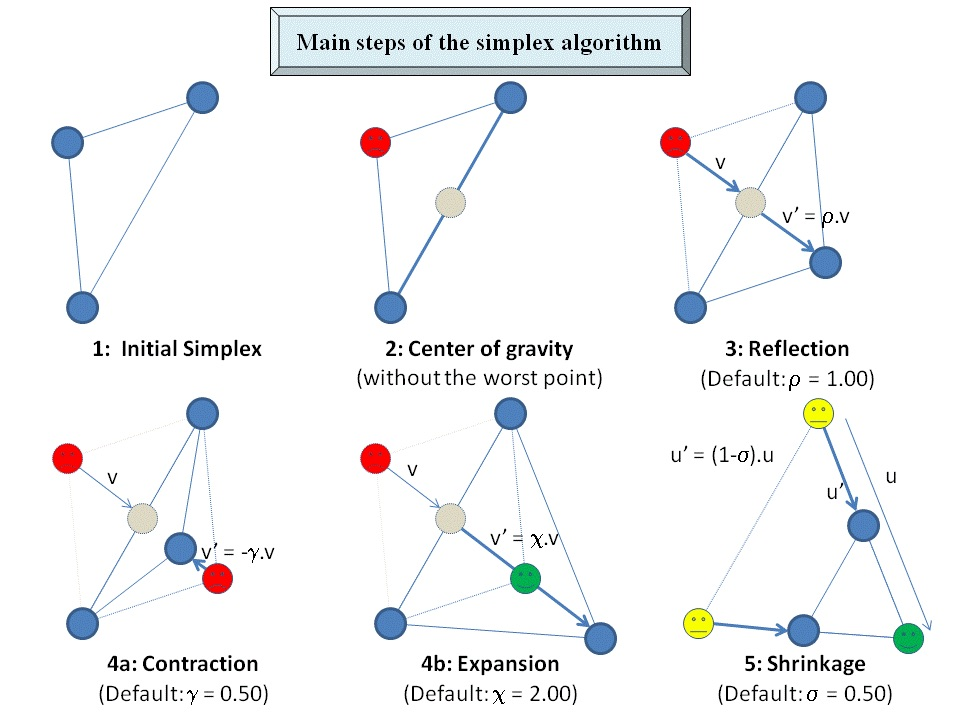
\includegraphics{../assets/figs/optimization/neldermeadsteps.jpg}

\begin{itemize}
\tightlist
\item
  this is a very popular method. The matlab functions \texttt{fmincon}
  and \texttt{fminsearch} implements it.
\item
  When it works, it works quite fast.
\item
  No derivatives required.
\end{itemize}

    \begin{Verbatim}[commandchars=\\\{\}]
{\color{incolor}In [{\color{incolor}20}]:} \PY{n}{optimize}\PY{p}{(}\PY{n}{rosenbrock}\PY{o}{.}\PY{n}{f}\PY{p}{,} \PY{p}{[}\PY{l+m+mf}{0.0}\PY{p}{,} \PY{l+m+mf}{0.0}\PY{p}{]}\PY{p}{,} \PY{n}{NelderMead}\PY{p}{(}\PY{p}{)}\PY{p}{)}
\end{Verbatim}


\begin{Verbatim}[commandchars=\\\{\}]
{\color{outcolor}Out[{\color{outcolor}20}]:} Results of Optimization Algorithm
          * Algorithm: Nelder-Mead
          * Starting Point: [0.0,0.0]
          * Minimizer: [0.9999634355313174,0.9999315506115275]
          * Minimum: 3.525527e-09
          * Iterations: 60
          * Convergence: true
            *  √(Σ(yᵢ-ȳ)²)/n < 1.0e-08: true
            * Reached Maximum Number of Iterations: false
          * Objective Calls: 117
\end{Verbatim}
            
    \begin{itemize}
\tightlist
\item
  But.
\end{itemize}

\subsection{Bracketing for Multidimensional Problems: Comment on
Nelder-Mead}\label{bracketing-for-multidimensional-problems-comment-on-nelder-mead}

\begin{quote}
Lagarias et al. (SIOPT, 1999): At present there is no function in any
dimension greater than one, for which the original Nelder-Mead algorithm
has been proved to converge to a minimizer.
\end{quote}

\begin{quote}
Given all the known inefficiencies and failures of the Nelder-Mead
algorithm {[}...{]}, one might wonder why it is used at all, let alone
why it is so extraordinarily popular.
\end{quote}

    \subsection{things to read up on}\label{things-to-read-up-on}

\begin{itemize}
\tightlist
\item
  Divided Rectangles (DIRECT)
\item
  simulated annealing and other stochastic gradient methods
\end{itemize}

    \subsection{Stochastic Optimization
Methods}\label{stochastic-optimization-methods}

\begin{itemize}
\tightlist
\item
  Gradient based methods like steepest descent may be susceptible to
  getting stuck at local minima.
\item
  Randomly shocking the value of the descent direction may be a solution
  to this.
\item
  For example, one could modify our gradient descent from before to
  become
\end{itemize}

\[\mathbf{x}^{(k+1)} \longleftarrow \mathbf{x}^{(k)} +\alpha^k\mathbf{g}^{(k)} + \mathbf{\varepsilon}^{(k)}\]

\begin{itemize}
\tightlist
\item
  where \(\mathbf{\varepsilon}^{(k)} \sim N(0,\sigma_k^2)\), decreasing
  with \(k\).
\item
  This \emph{stochastic gradient descent} is often used when training
  neural networks.
\end{itemize}

    \subsubsection{Simulated Annealing}\label{simulated-annealing}

\begin{itemize}
\tightlist
\item
  We specify a \emph{temperature} that controls the degree of
  randomness.
\item
  At first the temperature is high, letting the search jump around
  widely. This is to escape local minima.
\item
  The temperature is gradually decreased, reducing the step sizes. This
  is to find the local optimimum in the \emph{best} region.
\item
  At every iteration \(k\), we accept new point \(\mathbf{x'}\) with
\end{itemize}

\[
\Pr(\text{accept }\mathbf{x'}) = \begin{cases}
1 & \text{if }\Delta y \leq0 \\
\min(e^{\Delta y / t},1) & \text{if }\Delta y > 0 
\end{cases}
\]

\begin{itemize}
\tightlist
\item
  here \(\Delta y = f(\mathbf{x'}) - f(\mathbf{x})\), and \(t\) is the
  \emph{temperature}.
\item
  \(\Pr(\text{accept }\mathbf{x'})\) is called the \textbf{Metropolis
  Criterion}, building block of \emph{Accept/Reject} algorithms.
\end{itemize}

    \begin{Verbatim}[commandchars=\\\{\}]
{\color{incolor}In [{\color{incolor}21}]:} \PY{c}{\PYZsh{} f: function}
         \PY{c}{\PYZsh{} x: initial point}
         \PY{c}{\PYZsh{} T: transition distribution}
         \PY{c}{\PYZsh{} t: temp schedule, k\PYZus{}max: max iterations}
         \PY{k}{function} \PY{n}{simulated\PYZus{}annealing}\PY{p}{(}\PY{n}{f}\PY{p}{,} \PY{n}{x}\PY{p}{,} \PY{n}{T}\PY{p}{,} \PY{n}{t}\PY{p}{,} \PY{n}{k\PYZus{}max}\PY{p}{)} 
             \PY{n}{y} \PY{o}{=} \PY{n}{f}\PY{p}{(}\PY{n}{x}\PY{p}{)}
             \PY{n}{ytrace} \PY{o}{=} \PY{n}{zeros}\PY{p}{(}\PY{n}{typeof}\PY{p}{(}\PY{n}{y}\PY{p}{)}\PY{p}{,}\PY{n}{k\PYZus{}max}\PY{p}{)}
             \PY{n}{x\PYZus{}best}\PY{p}{,} \PY{n}{y\PYZus{}best} \PY{o}{=} \PY{n}{x}\PY{p}{,} \PY{n}{y} 
             \PY{k}{for} \PY{n}{k} \PY{k+kp}{in} \PY{l+m+mi}{1} \PY{o}{:} \PY{n}{k\PYZus{}max}
                 \PY{n}{x′} \PY{o}{=} \PY{n}{x} \PY{o}{+} \PY{n}{rand}\PY{p}{(}\PY{n}{T}\PY{p}{)}
                 \PY{n}{y′} \PY{o}{=} \PY{n}{f}\PY{p}{(}\PY{n}{x′}\PY{p}{)}
                 \PY{n}{Δy} \PY{o}{=} \PY{n}{y′} \PY{o}{\PYZhy{}} \PY{n}{y}
                 \PY{k}{if} \PY{n}{Δy} \PY{o}{≤} \PY{l+m+mi}{0} \PY{o}{||} \PY{n}{rand}\PY{p}{(}\PY{p}{)} \PY{o}{\PYZlt{}} \PY{n}{exp}\PY{p}{(}\PY{o}{\PYZhy{}}\PY{n}{Δy}\PY{o}{/}\PY{n}{t}\PY{p}{(}\PY{n}{k}\PY{p}{)}\PY{p}{)}
                     \PY{n}{x}\PY{p}{,} \PY{n}{y} \PY{o}{=} \PY{n}{x′}\PY{p}{,} \PY{n}{y′} 
                 \PY{k}{end}
                 \PY{k}{if} \PY{n}{y′} \PY{o}{\PYZlt{}} \PY{n}{y\PYZus{}best}
                     \PY{n}{x\PYZus{}best}\PY{p}{,} \PY{n}{y\PYZus{}best} \PY{o}{=} \PY{n}{x′}\PY{p}{,} \PY{n}{y′}
                 \PY{k}{end} 
                 \PY{n}{ytrace}\PY{p}{[}\PY{n}{k}\PY{p}{]} \PY{o}{=} \PY{n}{y\PYZus{}best}
             \PY{k}{end}
             \PY{k}{return} \PY{n}{x\PYZus{}best}\PY{p}{,}\PY{n}{ytrace}
         \PY{k}{end}
\end{Verbatim}


\begin{Verbatim}[commandchars=\\\{\}]
{\color{outcolor}Out[{\color{outcolor}21}]:} simulated\_annealing (generic function with 1 method)
\end{Verbatim}
            
    \begin{Verbatim}[commandchars=\\\{\}]
{\color{incolor}In [{\color{incolor}22}]:} \PY{k}{function} \PY{n}{ackley}\PY{p}{(}\PY{n}{x}\PY{p}{,} \PY{n}{a}\PY{o}{=}\PY{l+m+mi}{20}\PY{p}{,} \PY{n}{b}\PY{o}{=}\PY{l+m+mf}{0.2}\PY{p}{,} \PY{n}{c}\PY{o}{=}\PY{l+m+mi}{2}\PY{n+nb}{π}\PY{p}{)} 
             \PY{n}{d} \PY{o}{=} \PY{n}{length}\PY{p}{(}\PY{n}{x}\PY{p}{)}
             \PY{k}{return} \PY{o}{\PYZhy{}}\PY{n}{a}\PY{o}{*}\PY{n}{exp}\PY{p}{(}\PY{o}{\PYZhy{}}\PY{n}{b}\PY{o}{*}\PY{n}{sqrt}\PY{p}{(}\PY{n}{sum}\PY{p}{(}\PY{n}{x}\PY{o}{.\PYZca{}}\PY{l+m+mi}{2}\PY{p}{)}\PY{o}{/}\PY{n}{d}\PY{p}{)}\PY{p}{)} \PY{o}{\PYZhy{}} \PY{n}{exp}\PY{p}{(}\PY{n}{sum}\PY{p}{(}\PY{n}{cos}\PY{o}{.}\PY{p}{(}\PY{n}{c}\PY{o}{*}\PY{n}{xi}\PY{p}{)} \PY{k}{for} \PY{n}{xi} \PY{k+kp}{in} \PY{n}{x}\PY{p}{)}\PY{o}{/}\PY{n}{d}\PY{p}{)} \PY{o}{+} \PY{n}{a} \PY{o}{+} \PY{n+nb}{e}
         \PY{k}{end}
         \PY{k}{using} \PY{n}{Plots}
         \PY{n}{plotlyjs}\PY{p}{(}\PY{p}{)}
         \PY{n}{surface}\PY{p}{(}\PY{o}{\PYZhy{}}\PY{l+m+mi}{30}\PY{o}{:}\PY{l+m+mf}{0.1}\PY{o}{:}\PY{l+m+mi}{30}\PY{p}{,}\PY{o}{\PYZhy{}}\PY{l+m+mi}{30}\PY{o}{:}\PY{l+m+mf}{0.1}\PY{o}{:}\PY{l+m+mi}{30}\PY{p}{,}\PY{p}{(}\PY{n}{x}\PY{p}{,}\PY{n}{y}\PY{p}{)}\PY{o}{\PYZhy{}}\PY{o}{\PYZgt{}}\PY{n}{ackley}\PY{p}{(}\PY{p}{[}\PY{n}{x}\PY{p}{,} \PY{n}{y}\PY{p}{]}\PY{p}{)}\PY{p}{)}
\end{Verbatim}


    \begin{Verbatim}[commandchars=\\\{\}]
{\color{incolor}In [{\color{incolor}23}]:} \PY{k}{using} \PY{n}{Distributions}
         \PY{n}{d} \PY{o}{=} \PY{k+kt}{Dict}\PY{p}{(}\PY{p}{)}
         \PY{k}{for} \PY{n}{sig} \PY{k+kp}{in} \PY{p}{(}\PY{l+m+mi}{1}\PY{p}{,}\PY{l+m+mi}{5}\PY{p}{,}\PY{l+m+mi}{25}\PY{p}{)}\PY{p}{,} \PY{n}{t1} \PY{k+kp}{in} \PY{p}{(}\PY{l+m+mi}{1}\PY{p}{,}\PY{l+m+mi}{10}\PY{p}{,}\PY{l+m+mi}{25}\PY{p}{)}
             \PY{n}{tmp} \PY{o}{=} \PY{p}{[}\PY{n}{simulated\PYZus{}annealing}\PY{p}{(}\PY{n}{ackley}\PY{p}{,}\PY{p}{[}\PY{l+m+mi}{15}\PY{p}{,}\PY{l+m+mi}{15}\PY{p}{]}\PY{p}{,}\PY{n}{MvNormal}\PY{p}{(}\PY{l+m+mi}{2}\PY{p}{,}\PY{n}{sig}\PY{p}{)}\PY{p}{,}\PY{n}{x}\PY{o}{\PYZhy{}}\PY{o}{\PYZgt{}}\PY{n}{t1}\PY{o}{/}\PY{n}{x}\PY{p}{,}\PY{l+m+mi}{100}\PY{p}{)} \PY{k}{for} \PY{n}{i} \PY{k+kp}{in} \PY{l+m+mi}{1}\PY{o}{:}\PY{l+m+mi}{300}\PY{p}{]}
             \PY{n}{d}\PY{p}{[}\PY{p}{(}\PY{n}{sig}\PY{p}{,}\PY{n}{t1}\PY{p}{)}\PY{p}{]} \PY{o}{=} \PY{k+kt}{Dict}\PY{p}{(}\PY{p}{)}
             \PY{n}{d}\PY{p}{[}\PY{p}{(}\PY{n}{sig}\PY{p}{,}\PY{n}{t1}\PY{p}{)}\PY{p}{]}\PY{p}{[}\PY{o}{:}\PY{n}{y}\PY{p}{]} \PY{o}{=} \PY{n}{mapslices}\PY{p}{(}\PY{n}{x}\PY{o}{\PYZhy{}}\PY{o}{\PYZgt{}}\PY{n}{ackley}\PY{p}{(}\PY{n}{x}\PY{p}{)}\PY{p}{,}\PY{n}{hcat}\PY{p}{(}\PY{p}{[}\PY{n}{tmp}\PY{p}{[}\PY{n}{i}\PY{p}{]}\PY{p}{[}\PY{l+m+mi}{1}\PY{p}{]} \PY{k}{for} \PY{n}{i} \PY{k+kp}{in} \PY{l+m+mi}{1}\PY{o}{:}\PY{l+m+mi}{300}\PY{p}{]}\PY{o}{.}\PY{o}{.}\PY{o}{.}\PY{p}{)}\PY{p}{,}\PY{p}{[}\PY{l+m+mi}{1}\PY{p}{]}\PY{p}{)}
             \PY{n}{d}\PY{p}{[}\PY{p}{(}\PY{n}{sig}\PY{p}{,}\PY{n}{t1}\PY{p}{)}\PY{p}{]}\PY{p}{[}\PY{o}{:}\PY{n}{ytrace}\PY{p}{]} \PY{o}{=} \PY{n}{hcat}\PY{p}{(}\PY{p}{[}\PY{n}{tmp}\PY{p}{[}\PY{n}{i}\PY{p}{]}\PY{p}{[}\PY{l+m+mi}{2}\PY{p}{]} \PY{k}{for} \PY{n}{i} \PY{k+kp}{in} \PY{l+m+mi}{1}\PY{o}{:}\PY{l+m+mi}{300}\PY{p}{]}\PY{o}{.}\PY{o}{.}\PY{o}{.}\PY{p}{)}
         \PY{k}{end}
         
             
         \PY{c}{\PYZsh{} x=[simulated\PYZus{}annealing(ackley,[15,15],MvNormal(2,1),x\PYZhy{}\PYZgt{}1.0/x,100) for i in 1:100]}
         \PY{c}{\PYZsh{} y=[simulated\PYZus{}annealing(ackley,[15,15],MvNormal(2,5),x\PYZhy{}\PYZgt{}10.0/x,100) for i in 1:100]}
         \PY{c}{\PYZsh{} map((x)\PYZhy{}\PYZgt{}ackley([x[1],x[2] ]),y)}
\end{Verbatim}


    \section{Constraints}\label{constraints}

    \subsection{lagrange multipliers}\label{lagrange-multipliers}

    \subsection{duality}\label{duality}

    \subsection{~penalty methods}\label{penalty-methods}

    \subsection{~augmented lagrange}\label{augmented-lagrange}

    \subsection{~interior point}\label{interior-point}

    \subsubsection{Examples}\label{examples}

\[ 
\min_{x \in \mathbb{R}^2} \sqrt{x_2} \text{ subject to }\begin{array}{c} \\
 x_2 \geq 0 \\
 x_2 \geq (a_1 x_1 + b_1)^3 \\
x_2 \geq (a_2 x_1 + b_2)^3 
\end{array}
\]

    \subsection{\texorpdfstring{Constrained Optimisation with
\href{https://github.com/JuliaOpt/NLopt.jl}{\texttt{NLopt.jl}}}{Constrained Optimisation with NLopt.jl}}\label{constrained-optimisation-with-nlopt.jl}

\begin{itemize}
\tightlist
\item
  We need to specify one function for each objective and constraint.
\item
  Both of those functions need to compute the function value (i.e.
  objective or constraint) \emph{and} it's respective gradient.
\item
  \texttt{NLopt} expects contraints \textbf{always} to be formulated in
  the format \[ g(x) \leq 0 \] where \(g\) is your constraint function
\item
  The constraint function is formulated for each constraint at \(x\). it
  returns a number (the value of the constraint at \(x\)), and it fills
  out the gradient vector, which is the partial derivative of the
  current constraint wrt \(x\).
\item
  There is also the option to have vector valued constraints, see the
  documentation.
\item
  We set this up as follows:
\end{itemize}

    \begin{Verbatim}[commandchars=\\\{\}]
{\color{incolor}In [{\color{incolor}24}]:} \PY{k}{using} \PY{n}{NLopt}
         
         \PY{n}{count} \PY{o}{=} \PY{l+m+mi}{0} \PY{c}{\PYZsh{} keep track of \PYZsh{} function evaluations}
         
         \PY{k}{function} \PY{n}{myfunc}\PY{p}{(}\PY{n}{x}\PY{o}{::}\PY{k+kt}{Vector}\PY{p}{,} \PY{n}{grad}\PY{o}{::}\PY{k+kt}{Vector}\PY{p}{)}
             \PY{k}{if} \PY{n}{length}\PY{p}{(}\PY{n}{grad}\PY{p}{)} \PY{o}{\PYZgt{}} \PY{l+m+mi}{0}
                 \PY{n}{grad}\PY{p}{[}\PY{l+m+mi}{1}\PY{p}{]} \PY{o}{=} \PY{l+m+mi}{0}
                 \PY{n}{grad}\PY{p}{[}\PY{l+m+mi}{2}\PY{p}{]} \PY{o}{=} \PY{l+m+mf}{0.5}\PY{o}{/}\PY{n}{sqrt}\PY{p}{(}\PY{n}{x}\PY{p}{[}\PY{l+m+mi}{2}\PY{p}{]}\PY{p}{)}
             \PY{k}{end}
         
             \PY{k+kd}{global} \PY{n}{count}
             \PY{n}{count}\PY{o}{::}\PY{k+kt}{Int} \PY{o}{+=} \PY{l+m+mi}{1}
             \PY{n}{println}\PY{p}{(}\PY{l+s}{\PYZdq{}}\PY{l+s}{f}\PY{l+s}{\PYZus{}}\PY{l+s+si}{\PYZdl{}count}\PY{l+s}{(}\PY{l+s+si}{\PYZdl{}x}\PY{l+s}{)}\PY{l+s}{\PYZdq{}}\PY{p}{)}
         
             \PY{n}{sqrt}\PY{p}{(}\PY{n}{x}\PY{p}{[}\PY{l+m+mi}{2}\PY{p}{]}\PY{p}{)}
         \PY{k}{end}
         
         \PY{k}{function} \PY{n}{myconstraint}\PY{p}{(}\PY{n}{x}\PY{o}{::}\PY{k+kt}{Vector}\PY{p}{,} \PY{n}{grad}\PY{o}{::}\PY{k+kt}{Vector}\PY{p}{,} \PY{n}{a}\PY{p}{,} \PY{n}{b}\PY{p}{)}
             \PY{k}{if} \PY{n}{length}\PY{p}{(}\PY{n}{grad}\PY{p}{)} \PY{o}{\PYZgt{}} \PY{l+m+mi}{0}
                 \PY{n}{grad}\PY{p}{[}\PY{l+m+mi}{1}\PY{p}{]} \PY{o}{=} \PY{l+m+mi}{3}\PY{n}{a} \PY{o}{*} \PY{p}{(}\PY{n}{a}\PY{o}{*}\PY{n}{x}\PY{p}{[}\PY{l+m+mi}{1}\PY{p}{]} \PY{o}{+} \PY{n}{b}\PY{p}{)}\PY{o}{\PYZca{}}\PY{l+m+mi}{2}
                 \PY{n}{grad}\PY{p}{[}\PY{l+m+mi}{2}\PY{p}{]} \PY{o}{=} \PY{o}{\PYZhy{}}\PY{l+m+mi}{1}
             \PY{k}{end}
             \PY{p}{(}\PY{n}{a}\PY{o}{*}\PY{n}{x}\PY{p}{[}\PY{l+m+mi}{1}\PY{p}{]} \PY{o}{+} \PY{n}{b}\PY{p}{)}\PY{o}{\PYZca{}}\PY{l+m+mi}{3} \PY{o}{\PYZhy{}} \PY{n}{x}\PY{p}{[}\PY{l+m+mi}{2}\PY{p}{]}
         \PY{k}{end}
         
         \PY{n}{opt} \PY{o}{=} \PY{n}{Opt}\PY{p}{(}\PY{o}{:}\PY{n}{LD\PYZus{}MMA}\PY{p}{,} \PY{l+m+mi}{2}\PY{p}{)}
         \PY{n}{lower\PYZus{}bounds!}\PY{p}{(}\PY{n}{opt}\PY{p}{,} \PY{p}{[}\PY{o}{\PYZhy{}}\PY{n+nb}{Inf}\PY{p}{,} \PY{l+m+mf}{0.}\PY{p}{]}\PY{p}{)}
         \PY{n}{xtol\PYZus{}rel!}\PY{p}{(}\PY{n}{opt}\PY{p}{,}\PY{l+m+mf}{1e\PYZhy{}4}\PY{p}{)}
         
         \PY{n}{min\PYZus{}objective!}\PY{p}{(}\PY{n}{opt}\PY{p}{,} \PY{n}{myfunc}\PY{p}{)}
         \PY{n}{inequality\PYZus{}constraint!}\PY{p}{(}\PY{n}{opt}\PY{p}{,} \PY{p}{(}\PY{n}{x}\PY{p}{,}\PY{n}{g}\PY{p}{)} \PY{o}{\PYZhy{}}\PY{o}{\PYZgt{}} \PY{n}{myconstraint}\PY{p}{(}\PY{n}{x}\PY{p}{,}\PY{n}{g}\PY{p}{,}\PY{l+m+mi}{2}\PY{p}{,}\PY{l+m+mi}{0}\PY{p}{)}\PY{p}{,} \PY{l+m+mf}{1e\PYZhy{}8}\PY{p}{)}
         \PY{n}{inequality\PYZus{}constraint!}\PY{p}{(}\PY{n}{opt}\PY{p}{,} \PY{p}{(}\PY{n}{x}\PY{p}{,}\PY{n}{g}\PY{p}{)} \PY{o}{\PYZhy{}}\PY{o}{\PYZgt{}} \PY{n}{myconstraint}\PY{p}{(}\PY{n}{x}\PY{p}{,}\PY{n}{g}\PY{p}{,}\PY{o}{\PYZhy{}}\PY{l+m+mi}{1}\PY{p}{,}\PY{l+m+mi}{1}\PY{p}{)}\PY{p}{,} \PY{l+m+mf}{1e\PYZhy{}8}\PY{p}{)}
         
         \PY{p}{(}\PY{n}{minfn}\PY{p}{,}\PY{n}{minx}\PY{p}{,}\PY{n}{ret}\PY{p}{)} \PY{o}{=} \PY{n}{NLopt}\PY{o}{.}\PY{n}{optimize}\PY{p}{(}\PY{n}{opt}\PY{p}{,} \PY{p}{[}\PY{l+m+mf}{1.234}\PY{p}{,} \PY{l+m+mf}{5.678}\PY{p}{]}\PY{p}{)}
         \PY{n}{println}\PY{p}{(}\PY{l+s}{\PYZdq{}}\PY{l+s}{g}\PY{l+s}{o}\PY{l+s}{t}\PY{l+s}{ }\PY{l+s+si}{\PYZdl{}minf}\PY{l+s}{ }\PY{l+s}{a}\PY{l+s}{t}\PY{l+s}{ }\PY{l+s+si}{\PYZdl{}minx}\PY{l+s}{ }\PY{l+s}{a}\PY{l+s}{f}\PY{l+s}{t}\PY{l+s}{e}\PY{l+s}{r}\PY{l+s}{ }\PY{l+s+si}{\PYZdl{}count}\PY{l+s}{ }\PY{l+s}{i}\PY{l+s}{t}\PY{l+s}{e}\PY{l+s}{r}\PY{l+s}{a}\PY{l+s}{t}\PY{l+s}{i}\PY{l+s}{o}\PY{l+s}{n}\PY{l+s}{s}\PY{l+s}{ }\PY{l+s}{(}\PY{l+s}{r}\PY{l+s}{e}\PY{l+s}{t}\PY{l+s}{u}\PY{l+s}{r}\PY{l+s}{n}\PY{l+s}{e}\PY{l+s}{d}\PY{l+s}{ }\PY{l+s+si}{\PYZdl{}ret}\PY{l+s}{)}\PY{l+s}{\PYZdq{}}\PY{p}{)}
\end{Verbatim}


    \begin{Verbatim}[commandchars=\\\{\}]
\textcolor{ansi-cyan-intense}{\textbf{INFO: }}\textcolor{ansi-cyan}{Recompiling stale cache file /Users/florian.oswald/.julia/lib/v0.6/NLopt.ji for module NLopt.
}
    \end{Verbatim}

    \begin{Verbatim}[commandchars=\\\{\}]
f\_1([1.234, 5.678])
f\_2([0.878739, 5.55137])
f\_3([0.826216, 5.0439])
f\_4([0.473944, 4.07677])
f\_5([0.353898, 3.03085])
f\_6([0.333873, 1.97179])
f\_7([0.333334, 1.04509])
f\_8([0.333334, 0.469503])
f\_9([0.333333, 0.305792])
f\_10([0.333333, 0.296322])
f\_11([0.333333, 0.296296])
got minf at [0.333333, 0.296296] after 11 iterations (returned XTOL\_REACHED)

    \end{Verbatim}

    \begin{Verbatim}[commandchars=\\\{\}]
WARNING: using NLopt.optimize in module Main conflicts with an existing identifier.

    \end{Verbatim}

    \subsection{NLopt: Rosenbrock}\label{nlopt-rosenbrock}

\begin{itemize}
\tightlist
\item
  Let's tackle the rosenbrock example again.
\item
  To make it more interesting, let's add an inequality constraint.
  \[ \min_{x\in \mathbb{R}^2} (1-x_1)^2  + 100(x_2-x_1^2)^2  \text{  subject to  } 0.8 - x_1^2 -x_2^2 \geq 0 \]
\item
  in \texttt{NLopt} format, the constraint is \(x_1 + x_2 - 0.8 \leq 0\)
\end{itemize}

    \begin{Verbatim}[commandchars=\\\{\}]
{\color{incolor}In [{\color{incolor}25}]:} \PY{k}{function} \PY{n}{rosenbrockf}\PY{p}{(}\PY{n}{x}\PY{o}{::}\PY{k+kt}{Vector}\PY{p}{,}\PY{n}{grad}\PY{o}{::}\PY{k+kt}{Vector}\PY{p}{)}
             \PY{k}{if} \PY{n}{length}\PY{p}{(}\PY{n}{grad}\PY{p}{)} \PY{o}{\PYZgt{}} \PY{l+m+mi}{0}
         	    \PY{n}{grad}\PY{p}{[}\PY{l+m+mi}{1}\PY{p}{]} \PY{o}{=} \PY{o}{\PYZhy{}}\PY{l+m+mf}{2.0} \PY{o}{*} \PY{p}{(}\PY{l+m+mf}{1.0} \PY{o}{\PYZhy{}} \PY{n}{x}\PY{p}{[}\PY{l+m+mi}{1}\PY{p}{]}\PY{p}{)} \PY{o}{\PYZhy{}} \PY{l+m+mf}{400.0} \PY{o}{*} \PY{p}{(}\PY{n}{x}\PY{p}{[}\PY{l+m+mi}{2}\PY{p}{]} \PY{o}{\PYZhy{}} \PY{n}{x}\PY{p}{[}\PY{l+m+mi}{1}\PY{p}{]}\PY{o}{\PYZca{}}\PY{l+m+mi}{2}\PY{p}{)} \PY{o}{*} \PY{n}{x}\PY{p}{[}\PY{l+m+mi}{1}\PY{p}{]}
         	    \PY{n}{grad}\PY{p}{[}\PY{l+m+mi}{2}\PY{p}{]} \PY{o}{=} \PY{l+m+mf}{200.0} \PY{o}{*} \PY{p}{(}\PY{n}{x}\PY{p}{[}\PY{l+m+mi}{2}\PY{p}{]} \PY{o}{\PYZhy{}} \PY{n}{x}\PY{p}{[}\PY{l+m+mi}{1}\PY{p}{]}\PY{o}{\PYZca{}}\PY{l+m+mi}{2}\PY{p}{)}
             \PY{k}{end}
             \PY{k}{return} \PY{p}{(}\PY{l+m+mf}{1.0} \PY{o}{\PYZhy{}} \PY{n}{x}\PY{p}{[}\PY{l+m+mi}{1}\PY{p}{]}\PY{p}{)}\PY{o}{\PYZca{}}\PY{l+m+mi}{2} \PY{o}{+} \PY{l+m+mf}{100.0} \PY{o}{*} \PY{p}{(}\PY{n}{x}\PY{p}{[}\PY{l+m+mi}{2}\PY{p}{]} \PY{o}{\PYZhy{}} \PY{n}{x}\PY{p}{[}\PY{l+m+mi}{1}\PY{p}{]}\PY{o}{\PYZca{}}\PY{l+m+mi}{2}\PY{p}{)}\PY{o}{\PYZca{}}\PY{l+m+mi}{2}
         \PY{k}{end}
         \PY{k}{function} \PY{n}{r\PYZus{}constraint}\PY{p}{(}\PY{n}{x}\PY{o}{::}\PY{k+kt}{Vector}\PY{p}{,} \PY{n}{grad}\PY{o}{::}\PY{k+kt}{Vector}\PY{p}{)}
             \PY{k}{if} \PY{n}{length}\PY{p}{(}\PY{n}{grad}\PY{p}{)} \PY{o}{\PYZgt{}} \PY{l+m+mi}{0}
         	\PY{n}{grad}\PY{p}{[}\PY{l+m+mi}{1}\PY{p}{]} \PY{o}{=} \PY{l+m+mi}{2}\PY{o}{*}\PY{n}{x}\PY{p}{[}\PY{l+m+mi}{1}\PY{p}{]}
         	\PY{n}{grad}\PY{p}{[}\PY{l+m+mi}{2}\PY{p}{]} \PY{o}{=} \PY{l+m+mi}{2}\PY{o}{*}\PY{n}{x}\PY{p}{[}\PY{l+m+mi}{2}\PY{p}{]}
         	\PY{k}{end}
         	\PY{k}{return} \PY{n}{x}\PY{p}{[}\PY{l+m+mi}{1}\PY{p}{]}\PY{o}{\PYZca{}}\PY{l+m+mi}{2} \PY{o}{+} \PY{n}{x}\PY{p}{[}\PY{l+m+mi}{2}\PY{p}{]}\PY{o}{\PYZca{}}\PY{l+m+mi}{2} \PY{o}{\PYZhy{}} \PY{l+m+mf}{0.8}
         \PY{k}{end}
         \PY{n}{opt} \PY{o}{=} \PY{n}{Opt}\PY{p}{(}\PY{o}{:}\PY{n}{LD\PYZus{}MMA}\PY{p}{,} \PY{l+m+mi}{2}\PY{p}{)}
         \PY{n}{lower\PYZus{}bounds!}\PY{p}{(}\PY{n}{opt}\PY{p}{,} \PY{p}{[}\PY{o}{\PYZhy{}}\PY{l+m+mi}{5}\PY{p}{,} \PY{o}{\PYZhy{}}\PY{l+m+mf}{5.0}\PY{p}{]}\PY{p}{)}
         \PY{n}{min\PYZus{}objective!}\PY{p}{(}\PY{n}{opt}\PY{p}{,}\PY{p}{(}\PY{n}{x}\PY{p}{,}\PY{n}{g}\PY{p}{)} \PY{o}{\PYZhy{}}\PY{o}{\PYZgt{}} \PY{n}{rosenbrockf}\PY{p}{(}\PY{n}{x}\PY{p}{,}\PY{n}{g}\PY{p}{)}\PY{p}{)}
         \PY{n}{inequality\PYZus{}constraint!}\PY{p}{(}\PY{n}{opt}\PY{p}{,} \PY{p}{(}\PY{n}{x}\PY{p}{,}\PY{n}{g}\PY{p}{)} \PY{o}{\PYZhy{}}\PY{o}{\PYZgt{}} \PY{n}{r\PYZus{}constraint}\PY{p}{(}\PY{n}{x}\PY{p}{,}\PY{n}{g}\PY{p}{)}\PY{p}{)}
         \PY{n}{ftol\PYZus{}rel!}\PY{p}{(}\PY{n}{opt}\PY{p}{,}\PY{l+m+mf}{1e\PYZhy{}9}\PY{p}{)}
         \PY{n}{NLopt}\PY{o}{.}\PY{n}{optimize}\PY{p}{(}\PY{n}{opt}\PY{p}{,} \PY{p}{[}\PY{o}{\PYZhy{}}\PY{l+m+mf}{1.0}\PY{p}{,}\PY{l+m+mf}{0.0}\PY{p}{]}\PY{p}{)}
\end{Verbatim}


\begin{Verbatim}[commandchars=\\\{\}]
{\color{outcolor}Out[{\color{outcolor}25}]:} (0.07588358473630112, [0.724702, 0.524221], :FTOL\_REACHED)
\end{Verbatim}
            
    \subsection{JuMP.jl}\label{jump.jl}

\begin{itemize}
\tightlist
\item
  Introduce \href{https://github.com/JuliaOpt/JuMP.jl}{\texttt{JuMP.jl}}
\item
  JuMP is a mathematical programming interface for Julia. It is like
  AMPL, but for free and with a decent programming language.
\item
  The main highlights are:

  \begin{itemize}
  \tightlist
  \item
    It uses automatic differentiation to compute derivatives from your
    expression.
  \item
    It supplies this information, as well as the sparsity structure of
    the Hessian to your preferred solver.
  \item
    It decouples your problem completely from the type of solver you are
    using. This is great, since you don't have to worry about different
    solvers having different interfaces.
  \item
    In order to achieve this, \texttt{JuMP} uses
    \href{https://github.com/JuliaOpt/MathProgBase.jl}{\texttt{MathProgBase.jl}},
    which converts your problem formulation into a standard
    representation of an optimization problem.
  \end{itemize}
\item
  Let's look at the readme
\item
  The technical citation is Lubin et al \cite{JuMP}
\end{itemize}

    \subsection{JuMP: Quick start guide}\label{jump-quick-start-guide}

\begin{itemize}
\tightlist
\item
  this is form the
  \href{http://www.juliaopt.org/JuMP.jl/0.16/quickstart.html}{quick
  start guide}
\item
  please check the docs, they are excellent.
\end{itemize}

\subsubsection{Step 1: create a model}\label{step-1-create-a-model}

\begin{itemize}
\tightlist
\item
  A model collects variables, objective function and constraints.
\item
  it defines a solver to be used.
\end{itemize}

    \begin{Shaded}
\begin{Highlighting}[]
\NormalTok{using Clp}
\NormalTok{m = Model(solver=ClpSolver())  }\CommentTok{# provide a solver}

\CommentTok{# Define variables}
\NormalTok{@variable(m, x )              }\CommentTok{# No bounds}
\NormalTok{@variable(m, x >= lb )        }\CommentTok{# Lower bound only (note: 'lb <= x' is not valid)}
\NormalTok{@variable(m, x <= ub )        }\CommentTok{# Upper bound only}
\NormalTok{@variable(m, lb <= x <= ub )  }\CommentTok{# Lower and upper bounds}
\end{Highlighting}
\end{Shaded}

    \begin{Shaded}
\begin{Highlighting}[]

\CommentTok{# we can create arrays of a variable}
\NormalTok{N = }\FloatTok{2}
\NormalTok{@variable(m, x[}\FloatTok{1}\NormalTok{:M,}\FloatTok{1}\NormalTok{:N] >= }\FloatTok{0} \NormalTok{)}

\CommentTok{# or put them in a block}
\NormalTok{@variables m }\KeywordTok{begin}
    \NormalTok{x}
    \NormalTok{y >= }\FloatTok{0}
    \NormalTok{Z[}\FloatTok{1}\NormalTok{:}\FloatTok{10}\NormalTok{], Bin}
    \NormalTok{X[}\FloatTok{1}\NormalTok{:}\FloatTok{3}\NormalTok{,}\FloatTok{1}\NormalTok{:}\FloatTok{3}\NormalTok{], SDP}
    \NormalTok{q[i=}\FloatTok{1}\NormalTok{:}\FloatTok{2}\NormalTok{], (lowerbound = i, start = }\FloatTok{2}\NormalTok{i, upperbound = }\FloatTok{3}\NormalTok{i)}
    \NormalTok{t[j=}\FloatTok{1}\NormalTok{:}\FloatTok{3}\NormalTok{], (}\DataTypeTok{Int}\NormalTok{, start = j)}
\KeywordTok{end}

\CommentTok{# Equivalent to:}
\NormalTok{@variable(m, x)}
\NormalTok{@variable(m, y >= }\FloatTok{0}\NormalTok{)}
\NormalTok{@variable(m, Z[}\FloatTok{1}\NormalTok{:}\FloatTok{10}\NormalTok{], Bin)}
\NormalTok{@variable(m, X[}\FloatTok{1}\NormalTok{:}\FloatTok{3}\NormalTok{,}\FloatTok{1}\NormalTok{:}\FloatTok{3}\NormalTok{], SDP)}
\NormalTok{@variable(m, q[i=}\FloatTok{1}\NormalTok{:}\FloatTok{2}\NormalTok{], lowerbound = i, start = }\FloatTok{2}\NormalTok{i, upperbound = }\FloatTok{3}\NormalTok{i)}
\NormalTok{@variable(m, t[j=}\FloatTok{1}\NormalTok{:}\FloatTok{3}\NormalTok{], }\DataTypeTok{Int}\NormalTok{, start = j)}

\CommentTok{# bounds can depend on indices}
\NormalTok{@variable(m, x[i=}\FloatTok{1}\NormalTok{:}\FloatTok{10}\NormalTok{] >= i )}
\end{Highlighting}
\end{Shaded}

    \subsection{Objective and Constraints}\label{objective-and-constraints}

\begin{itemize}
\tightlist
\item
  We can easily add objective and constraint functions:
\end{itemize}

\begin{Shaded}
\begin{Highlighting}[]
\NormalTok{@constraint(m, x[i] - s[i] <= }\FloatTok{0}\NormalTok{)  }\CommentTok{# Other options: == and >=}
\NormalTok{@constraint(m, sum(x[i] }\KeywordTok{for} \NormalTok{i=}\FloatTok{1}\NormalTok{:numLocation) == }\FloatTok{1}\NormalTok{)}
\NormalTok{@objective(m, Max, }\FloatTok{5}\NormalTok{x + }\FloatTok{22}\NormalTok{y + (x+y)/}\FloatTok{2}\NormalTok{) }\CommentTok{# or Min}
\end{Highlighting}
\end{Shaded}

\begin{itemize}
\tightlist
\item
  This is fully integrated with Julia. you can use the
  \texttt{generator} syntax for sums:
\end{itemize}

\begin{Shaded}
\begin{Highlighting}[]
\NormalTok{@objective(sum(x[i] + y[i]/pi }\KeywordTok{for} \NormalTok{i = I1, j = I2 }\KeywordTok{if} \NormalTok{i+j < some_val))}
\end{Highlighting}
\end{Shaded}

    \begin{Verbatim}[commandchars=\\\{\}]
{\color{incolor}In [{\color{incolor}26}]:} \PY{c}{\PYZsh{}\PYZsh{} Simple example}
         \PY{k}{using} \PY{n}{JuMP}
         \PY{k}{using} \PY{n}{Clp}
         
         \PY{n}{m} \PY{o}{=} \PY{n}{Model}\PY{p}{(}\PY{n}{solver} \PY{o}{=} \PY{n}{ClpSolver}\PY{p}{(}\PY{p}{)}\PY{p}{)}
         \PY{n+nd}{@variable}\PY{p}{(}\PY{n}{m}\PY{p}{,} \PY{l+m+mi}{0} \PY{o}{\PYZlt{}=} \PY{n}{x} \PY{o}{\PYZlt{}=} \PY{l+m+mi}{2} \PY{p}{)}
         \PY{n+nd}{@variable}\PY{p}{(}\PY{n}{m}\PY{p}{,} \PY{l+m+mi}{0} \PY{o}{\PYZlt{}=} \PY{n}{y} \PY{o}{\PYZlt{}=} \PY{l+m+mi}{30} \PY{p}{)}
         
         \PY{n+nd}{@objective}\PY{p}{(}\PY{n}{m}\PY{p}{,} \PY{n}{Max}\PY{p}{,} \PY{l+m+mi}{5}\PY{n}{x} \PY{o}{+} \PY{l+m+mi}{3}\PY{o}{*}\PY{n}{y} \PY{p}{)}
         \PY{n+nd}{@constraint}\PY{p}{(}\PY{n}{m}\PY{p}{,} \PY{l+m+mi}{1}\PY{n}{x} \PY{o}{+} \PY{l+m+mi}{5}\PY{n}{y} \PY{o}{\PYZlt{}=} \PY{l+m+mf}{3.0} \PY{p}{)}
         
         \PY{n}{print}\PY{p}{(}\PY{n}{m}\PY{p}{)}
         
         \PY{n}{status} \PY{o}{=} \PY{n}{solve}\PY{p}{(}\PY{n}{m}\PY{p}{)}
         
         \PY{n}{println}\PY{p}{(}\PY{l+s}{\PYZdq{}}\PY{l+s}{O}\PY{l+s}{b}\PY{l+s}{j}\PY{l+s}{e}\PY{l+s}{c}\PY{l+s}{t}\PY{l+s}{i}\PY{l+s}{v}\PY{l+s}{e}\PY{l+s}{ }\PY{l+s}{v}\PY{l+s}{a}\PY{l+s}{l}\PY{l+s}{u}\PY{l+s}{e}\PY{l+s}{:}\PY{l+s}{ }\PY{l+s}{\PYZdq{}}\PY{p}{,} \PY{n}{getobjectivevalue}\PY{p}{(}\PY{n}{m}\PY{p}{)}\PY{p}{)}
         \PY{n}{println}\PY{p}{(}\PY{l+s}{\PYZdq{}}\PY{l+s}{x}\PY{l+s}{ }\PY{l+s}{=}\PY{l+s}{ }\PY{l+s}{\PYZdq{}}\PY{p}{,} \PY{n}{getvalue}\PY{p}{(}\PY{n}{x}\PY{p}{)}\PY{p}{)}
         \PY{n}{println}\PY{p}{(}\PY{l+s}{\PYZdq{}}\PY{l+s}{y}\PY{l+s}{ }\PY{l+s}{=}\PY{l+s}{ }\PY{l+s}{\PYZdq{}}\PY{p}{,} \PY{n}{getvalue}\PY{p}{(}\PY{n}{y}\PY{p}{)}\PY{p}{)}
\end{Verbatim}


    \begin{Verbatim}[commandchars=\\\{\}]
\textcolor{ansi-cyan-intense}{\textbf{INFO: }}\textcolor{ansi-cyan}{Recompiling stale cache file /Users/florian.oswald/.julia/lib/v0.6/Clp.ji for module Clp.
}
    \end{Verbatim}

    \begin{Verbatim}[commandchars=\\\{\}]
Max 5 x + 3 y
Subject to
 x + 5 y ≤ 3
 0 ≤ x ≤ 2
 0 ≤ y ≤ 30
Objective value: 10.6
x = 2.0
y = 0.2

    \end{Verbatim}

    \begin{Verbatim}[commandchars=\\\{\}]
{\color{incolor}In [{\color{incolor}27}]:} \PY{c}{\PYZsh{} JuMP: Rosenbrock Example}
         \PY{c}{\PYZsh{} Instead of hand\PYZhy{}coding first and second derivatives, you only have to give `JuMP` expressions for objective and constraints.}
         \PY{c}{\PYZsh{} Here is an example.}
         
         \PY{k}{using} \PY{n}{Ipopt}
         
         \PY{k}{let}
         
             \PY{n}{m} \PY{o}{=} \PY{n}{Model}\PY{p}{(}\PY{n}{solver}\PY{o}{=}\PY{n}{IpoptSolver}\PY{p}{(}\PY{p}{)}\PY{p}{)}
         
             \PY{n+nd}{@variable}\PY{p}{(}\PY{n}{m}\PY{p}{,} \PY{n}{x}\PY{p}{)}
             \PY{n+nd}{@variable}\PY{p}{(}\PY{n}{m}\PY{p}{,} \PY{n}{y}\PY{p}{)}
         
             \PY{n+nd}{@NLobjective}\PY{p}{(}\PY{n}{m}\PY{p}{,} \PY{n}{Min}\PY{p}{,} \PY{p}{(}\PY{l+m+mi}{1}\PY{o}{\PYZhy{}}\PY{n}{x}\PY{p}{)}\PY{o}{\PYZca{}}\PY{l+m+mi}{2} \PY{o}{+} \PY{l+m+mi}{100}\PY{p}{(}\PY{n}{y}\PY{o}{\PYZhy{}}\PY{n}{x}\PY{o}{\PYZca{}}\PY{l+m+mi}{2}\PY{p}{)}\PY{o}{\PYZca{}}\PY{l+m+mi}{2}\PY{p}{)}
         
             \PY{n}{solve}\PY{p}{(}\PY{n}{m}\PY{p}{)}
         
             \PY{n}{println}\PY{p}{(}\PY{l+s}{\PYZdq{}}\PY{l+s}{x}\PY{l+s}{ }\PY{l+s}{=}\PY{l+s}{ }\PY{l+s}{\PYZdq{}}\PY{p}{,} \PY{n}{getvalue}\PY{p}{(}\PY{n}{x}\PY{p}{)}\PY{p}{,} \PY{l+s}{\PYZdq{}}\PY{l+s}{ }\PY{l+s}{y}\PY{l+s}{ }\PY{l+s}{=}\PY{l+s}{ }\PY{l+s}{\PYZdq{}}\PY{p}{,} \PY{n}{getvalue}\PY{p}{(}\PY{n}{y}\PY{p}{)}\PY{p}{)}
         
         \PY{k}{end}
\end{Verbatim}


    \begin{Verbatim}[commandchars=\\\{\}]

******************************************************************************
This program contains Ipopt, a library for large-scale nonlinear optimization.
 Ipopt is released as open source code under the Eclipse Public License (EPL).
         For more information visit http://projects.coin-or.org/Ipopt
******************************************************************************

This is Ipopt version 3.12.8, running with linear solver mumps.
NOTE: Other linear solvers might be more efficient (see Ipopt documentation).

Number of nonzeros in equality constraint Jacobian{\ldots}:        0
Number of nonzeros in inequality constraint Jacobian.:        0
Number of nonzeros in Lagrangian Hessian{\ldots}:        3

Total number of variables{\ldots}:        2
                     variables with only lower bounds:        0
                variables with lower and upper bounds:        0
                     variables with only upper bounds:        0
Total number of equality constraints{\ldots}:        0
Total number of inequality constraints{\ldots}:        0
        inequality constraints with only lower bounds:        0
   inequality constraints with lower and upper bounds:        0
        inequality constraints with only upper bounds:        0

iter    objective    inf\_pr   inf\_du lg(mu)  ||d||  lg(rg) alpha\_du alpha\_pr  ls
   0  1.0000000e+00 0.00e+00 2.00e+00  -1.0 0.00e+00    -  0.00e+00 0.00e+00   0
   1  9.5312500e-01 0.00e+00 1.25e+01  -1.0 1.00e+00    -  1.00e+00 2.50e-01f  3
   2  4.8320569e-01 0.00e+00 1.01e+00  -1.0 9.03e-02    -  1.00e+00 1.00e+00f  1
   3  4.5708829e-01 0.00e+00 9.53e+00  -1.0 4.29e-01    -  1.00e+00 5.00e-01f  2
   4  1.8894205e-01 0.00e+00 4.15e-01  -1.0 9.51e-02    -  1.00e+00 1.00e+00f  1
   5  1.3918726e-01 0.00e+00 6.51e+00  -1.7 3.49e-01    -  1.00e+00 5.00e-01f  2
   6  5.4940990e-02 0.00e+00 4.51e-01  -1.7 9.29e-02    -  1.00e+00 1.00e+00f  1
   7  2.9144630e-02 0.00e+00 2.27e+00  -1.7 2.49e-01    -  1.00e+00 5.00e-01f  2
   8  9.8586451e-03 0.00e+00 1.15e+00  -1.7 1.10e-01    -  1.00e+00 1.00e+00f  1
   9  2.3237475e-03 0.00e+00 1.00e+00  -1.7 1.00e-01    -  1.00e+00 1.00e+00f  1
iter    objective    inf\_pr   inf\_du lg(mu)  ||d||  lg(rg) alpha\_du alpha\_pr  ls
  10  2.3797236e-04 0.00e+00 2.19e-01  -1.7 5.09e-02    -  1.00e+00 1.00e+00f  1
  11  4.9267371e-06 0.00e+00 5.95e-02  -1.7 2.53e-02    -  1.00e+00 1.00e+00f  1
  12  2.8189505e-09 0.00e+00 8.31e-04  -2.5 3.20e-03    -  1.00e+00 1.00e+00f  1
  13  1.0095040e-15 0.00e+00 8.68e-07  -5.7 9.78e-05    -  1.00e+00 1.00e+00f  1
  14  1.3288608e-28 0.00e+00 2.02e-13  -8.6 4.65e-08    -  1.00e+00 1.00e+00f  1

Number of Iterations{\ldots}: 14

                                   (scaled)                 (unscaled)
Objective{\ldots}:   1.3288608467480825e-28    1.3288608467480825e-28
Dual infeasibility{\ldots}:   2.0183854587685121e-13    2.0183854587685121e-13
Constraint violation{\ldots}:   0.0000000000000000e+00    0.0000000000000000e+00
Complementarity{\ldots}:   0.0000000000000000e+00    0.0000000000000000e+00
Overall NLP error{\ldots}:   2.0183854587685121e-13    2.0183854587685121e-13


Number of objective function evaluations             = 36
Number of objective gradient evaluations             = 15
Number of equality constraint evaluations            = 0
Number of inequality constraint evaluations          = 0
Number of equality constraint Jacobian evaluations   = 0
Number of inequality constraint Jacobian evaluations = 0
Number of Lagrangian Hessian evaluations             = 14
Total CPU secs in IPOPT (w/o function evaluations)   =      0.180
Total CPU secs in NLP function evaluations           =      0.030

EXIT: Optimal Solution Found.
x = 0.9999999999999899 y = 0.9999999999999792

    \end{Verbatim}

    \begin{Verbatim}[commandchars=\\\{\}]
{\color{incolor}In [{\color{incolor}28}]:} \PY{c}{\PYZsh{} not bad, right?}
         \PY{c}{\PYZsh{} adding the constraint from before:}
         
         \PY{k}{let}
             
             \PY{n}{m} \PY{o}{=} \PY{n}{Model}\PY{p}{(}\PY{n}{solver}\PY{o}{=}\PY{n}{IpoptSolver}\PY{p}{(}\PY{p}{)}\PY{p}{)}
         
             \PY{n+nd}{@variable}\PY{p}{(}\PY{n}{m}\PY{p}{,} \PY{n}{x}\PY{p}{)}
             \PY{n+nd}{@variable}\PY{p}{(}\PY{n}{m}\PY{p}{,} \PY{n}{y}\PY{p}{)}
         
             \PY{n+nd}{@NLobjective}\PY{p}{(}\PY{n}{m}\PY{p}{,} \PY{n}{Min}\PY{p}{,} \PY{p}{(}\PY{l+m+mi}{1}\PY{o}{\PYZhy{}}\PY{n}{x}\PY{p}{)}\PY{o}{\PYZca{}}\PY{l+m+mi}{2} \PY{o}{+} \PY{l+m+mi}{100}\PY{p}{(}\PY{n}{y}\PY{o}{\PYZhy{}}\PY{n}{x}\PY{o}{\PYZca{}}\PY{l+m+mi}{2}\PY{p}{)}\PY{o}{\PYZca{}}\PY{l+m+mi}{2}\PY{p}{)}
             \PY{n+nd}{@NLconstraint}\PY{p}{(}\PY{n}{m}\PY{p}{,}\PY{n}{x}\PY{o}{\PYZca{}}\PY{l+m+mi}{2} \PY{o}{+} \PY{n}{y}\PY{o}{\PYZca{}}\PY{l+m+mi}{2} \PY{o}{\PYZlt{}=} \PY{l+m+mf}{0.8}\PY{p}{)}
         
             \PY{n}{solve}\PY{p}{(}\PY{n}{m}\PY{p}{)}
         
             \PY{n}{println}\PY{p}{(}\PY{l+s}{\PYZdq{}}\PY{l+s}{x}\PY{l+s}{ }\PY{l+s}{=}\PY{l+s}{ }\PY{l+s}{\PYZdq{}}\PY{p}{,} \PY{n}{getvalue}\PY{p}{(}\PY{n}{x}\PY{p}{)}\PY{p}{,} \PY{l+s}{\PYZdq{}}\PY{l+s}{ }\PY{l+s}{y}\PY{l+s}{ }\PY{l+s}{=}\PY{l+s}{ }\PY{l+s}{\PYZdq{}}\PY{p}{,} \PY{n}{getvalue}\PY{p}{(}\PY{n}{y}\PY{p}{)}\PY{p}{)}
         
         \PY{k}{end}
\end{Verbatim}


    \begin{Verbatim}[commandchars=\\\{\}]
This is Ipopt version 3.12.8, running with linear solver mumps.
NOTE: Other linear solvers might be more efficient (see Ipopt documentation).

Number of nonzeros in equality constraint Jacobian{\ldots}:        0
Number of nonzeros in inequality constraint Jacobian.:        2
Number of nonzeros in Lagrangian Hessian{\ldots}:        5

Total number of variables{\ldots}:        2
                     variables with only lower bounds:        0
                variables with lower and upper bounds:        0
                     variables with only upper bounds:        0
Total number of equality constraints{\ldots}:        0
Total number of inequality constraints{\ldots}:        1
        inequality constraints with only lower bounds:        0
   inequality constraints with lower and upper bounds:        0
        inequality constraints with only upper bounds:        1

iter    objective    inf\_pr   inf\_du lg(mu)  ||d||  lg(rg) alpha\_du alpha\_pr  ls
   0  1.0000000e+00 0.00e+00 2.00e+00  -1.0 0.00e+00    -  0.00e+00 0.00e+00   0
   1  9.5312500e-01 0.00e+00 1.25e+01  -1.0 5.00e-01    -  1.00e+00 5.00e-01f  2
   2  4.9204994e-01 0.00e+00 9.72e-01  -1.0 8.71e-02    -  1.00e+00 1.00e+00f  1
   3  2.0451702e+00 0.00e+00 3.69e+01  -1.7 3.80e-01    -  1.00e+00 1.00e+00H  1
   4  1.0409466e-01 0.00e+00 3.10e-01  -1.7 1.46e-01    -  1.00e+00 1.00e+00f  1
   5  8.5804626e-02 0.00e+00 2.71e-01  -1.7 9.98e-02    -  1.00e+00 1.00e+00h  1
   6  9.4244879e-02 0.00e+00 6.24e-02  -1.7 3.74e-02    -  1.00e+00 1.00e+00h  1
   7  8.0582034e-02 0.00e+00 1.51e-01  -2.5 6.41e-02    -  1.00e+00 1.00e+00h  1
   8  7.8681242e-02 0.00e+00 2.12e-03  -2.5 1.12e-02    -  1.00e+00 1.00e+00h  1
   9  7.6095770e-02 0.00e+00 6.16e-03  -3.8 1.37e-02    -  1.00e+00 1.00e+00h  1
iter    objective    inf\_pr   inf\_du lg(mu)  ||d||  lg(rg) alpha\_du alpha\_pr  ls
  10  7.6033892e-02 0.00e+00 2.23e-06  -3.8 3.99e-04    -  1.00e+00 1.00e+00h  1
  11  7.5885642e-02 0.00e+00 2.07e-05  -5.7 7.99e-04    -  1.00e+00 1.00e+00h  1
  12  7.5885428e-02 0.00e+00 2.74e-11  -5.7 1.38e-06    -  1.00e+00 1.00e+00h  1
  13  7.5883585e-02 0.00e+00 3.19e-09  -8.6 9.93e-06    -  1.00e+00 1.00e+00f  1

Number of Iterations{\ldots}: 13

                                   (scaled)                 (unscaled)
Objective{\ldots}:   7.5883585442440671e-02    7.5883585442440671e-02
Dual infeasibility{\ldots}:   3.1949178858070582e-09    3.1949178858070582e-09
Constraint violation{\ldots}:   0.0000000000000000e+00    0.0000000000000000e+00
Complementarity{\ldots}:   2.5454985882932001e-09    2.5454985882932001e-09
Overall NLP error{\ldots}:   3.1949178858070582e-09    3.1949178858070582e-09


Number of objective function evaluations             = 20
Number of objective gradient evaluations             = 14
Number of equality constraint evaluations            = 0
Number of inequality constraint evaluations          = 20
Number of equality constraint Jacobian evaluations   = 0
Number of inequality constraint Jacobian evaluations = 14
Number of Lagrangian Hessian evaluations             = 13
Total CPU secs in IPOPT (w/o function evaluations)   =      0.006
Total CPU secs in NLP function evaluations           =      0.004

EXIT: Optimal Solution Found.
x = 0.7247018392092258 y = 0.5242206029480763

    \end{Verbatim}

    \subsection{JuMP: Maximium Likelihood}\label{jump-maximium-likelihood}

\begin{itemize}
\tightlist
\item
  Let's redo the maximum likelihood example in JuMP.
\item
  Let \(\mu,\sigma^2\) be the unknown mean and variance of a random
  sample generated from the normal distribution.
\item
  Find the maximum likelihood estimator for those parameters!
\item
  density:
\end{itemize}

\[ f(x_i|\mu,\sigma^2) = \frac{1}{\sigma \sqrt{2\pi}} \exp\left(-\frac{(x_i - \mu)^2}{2\sigma^2}\right) 
\]

\begin{itemize}
\tightlist
\item
  Likelihood Function
\end{itemize}

\[ \begin{aligned} 
L(\mu,\sigma^2) = \Pi_{i=1}^N f(x_i|\mu,\sigma^2) =& \frac{1}{(\sigma \sqrt{2\pi})^n} \exp\left(-\frac{1}{2\sigma^2} \sum_{i=1}^N (x_i-\mu)^2 \right) \\
     =& \left(\sigma^2 2\pi\right)^{-\frac{n}{2}} \exp\left(-\frac{1}{2\sigma^2} \sum_{i=1}^N (x_i-\mu)^2 \right) 
\end{aligned} 
\]

\begin{itemize}
\tightlist
\item
  Constraints: \(\mu\in \mathbb{R},\sigma>0\)
\item
  log-likelihood:
\end{itemize}

\[ \log L = l = -\frac{n}{2} \log \left( 2\pi \sigma^2 \right) - \frac{1}{2\sigma^2} \sum_{i=1}^N (x_i-\mu)^2 \]

\begin{itemize}
\tightlist
\item
  Let's do this in \texttt{JuMP}.
\end{itemize}

    \begin{Verbatim}[commandchars=\\\{\}]
{\color{incolor}In [{\color{incolor}29}]:} \PY{c}{\PYZsh{}  Copyright 2015, Iain Dunning, Joey Huchette, Miles Lubin, and contributors}
         \PY{c}{\PYZsh{}  example modified }
         \PY{k}{using} \PY{n}{Distributions}
         
         \PY{n}{distrib} \PY{o}{=} \PY{n}{Normal}\PY{p}{(}\PY{l+m+mf}{4.5}\PY{p}{,}\PY{l+m+mf}{3.5}\PY{p}{)}
         \PY{n}{n} \PY{o}{=} \PY{l+m+mi}{10000}
         
         \PY{n}{data} \PY{o}{=} \PY{n}{rand}\PY{p}{(}\PY{n}{distrib}\PY{p}{,}\PY{n}{n}\PY{p}{)}\PY{p}{;}
         
         \PY{n}{m} \PY{o}{=} \PY{n}{Model}\PY{p}{(}\PY{n}{solver}\PY{o}{=}\PY{n}{IpoptSolver}\PY{p}{(}\PY{p}{)}\PY{p}{)}
         
         \PY{n+nd}{@variable}\PY{p}{(}\PY{n}{m}\PY{p}{,} \PY{n}{mu}\PY{p}{,} \PY{n}{start} \PY{o}{=} \PY{l+m+mf}{0.0}\PY{p}{)}
         \PY{n+nd}{@variable}\PY{p}{(}\PY{n}{m}\PY{p}{,} \PY{n}{sigma} \PY{o}{\PYZgt{}=} \PY{l+m+mf}{0.0}\PY{p}{,} \PY{n}{start} \PY{o}{=} \PY{l+m+mf}{1.0}\PY{p}{)}
         
         \PY{n+nd}{@NLobjective}\PY{p}{(}\PY{n}{m}\PY{p}{,} \PY{n}{Max}\PY{p}{,} \PY{o}{\PYZhy{}}\PY{p}{(}\PY{n}{n}\PY{o}{/}\PY{l+m+mi}{2}\PY{p}{)}\PY{o}{*}\PY{n}{log}\PY{p}{(}\PY{l+m+mi}{2}\PY{n+nb}{π}\PY{o}{*}\PY{n}{sigma}\PY{o}{\PYZca{}}\PY{l+m+mi}{2}\PY{p}{)}\PY{o}{\PYZhy{}}\PY{n}{sum}\PY{p}{(}\PY{p}{(}\PY{n}{data}\PY{p}{[}\PY{n}{i}\PY{p}{]} \PY{o}{\PYZhy{}} \PY{n}{mu}\PY{p}{)} \PY{o}{\PYZca{}} \PY{l+m+mi}{2} \PY{k}{for} \PY{n}{i} \PY{o}{=} \PY{l+m+mi}{1}\PY{o}{:}\PY{n}{n}\PY{p}{)}\PY{o}{/}\PY{p}{(}\PY{l+m+mi}{2}\PY{o}{*}\PY{n}{sigma}\PY{o}{\PYZca{}}\PY{l+m+mi}{2}\PY{p}{)}\PY{p}{)}
         
         \PY{n}{solve}\PY{p}{(}\PY{n}{m}\PY{p}{)}
         \PY{n}{println}\PY{p}{(}\PY{l+s}{\PYZdq{}}\PY{l+s}{μ}\PY{l+s}{ }\PY{l+s}{=}\PY{l+s}{ }\PY{l+s}{\PYZdq{}}\PY{p}{,} \PY{n}{getvalue}\PY{p}{(}\PY{n}{mu}\PY{p}{)}\PY{p}{,}\PY{l+s}{\PYZdq{}}\PY{l+s}{,}\PY{l+s}{ }\PY{l+s}{m}\PY{l+s}{e}\PY{l+s}{a}\PY{l+s}{n}\PY{l+s}{(}\PY{l+s}{d}\PY{l+s}{a}\PY{l+s}{t}\PY{l+s}{a}\PY{l+s}{)}\PY{l+s}{ }\PY{l+s}{=}\PY{l+s}{ }\PY{l+s}{\PYZdq{}}\PY{p}{,} \PY{n}{mean}\PY{p}{(}\PY{n}{data}\PY{p}{)}\PY{p}{)}
         \PY{n}{println}\PY{p}{(}\PY{l+s}{\PYZdq{}}\PY{l+s}{σ}\PY{l+s}{\PYZca{}}\PY{l+s}{2}\PY{l+s}{ }\PY{l+s}{=}\PY{l+s}{ }\PY{l+s}{\PYZdq{}}\PY{p}{,} \PY{n}{getvalue}\PY{p}{(}\PY{n}{sigma}\PY{p}{)}\PY{o}{\PYZca{}}\PY{l+m+mi}{2}\PY{p}{,} \PY{l+s}{\PYZdq{}}\PY{l+s}{,}\PY{l+s}{ }\PY{l+s}{v}\PY{l+s}{a}\PY{l+s}{r}\PY{l+s}{(}\PY{l+s}{d}\PY{l+s}{a}\PY{l+s}{t}\PY{l+s}{a}\PY{l+s}{)}\PY{l+s}{ }\PY{l+s}{=}\PY{l+s}{ }\PY{l+s}{\PYZdq{}}\PY{p}{,} \PY{n}{var}\PY{p}{(}\PY{n}{data}\PY{p}{)}\PY{p}{)}
\end{Verbatim}


    \begin{Verbatim}[commandchars=\\\{\}]
This is Ipopt version 3.12.8, running with linear solver mumps.
NOTE: Other linear solvers might be more efficient (see Ipopt documentation).

Number of nonzeros in equality constraint Jacobian{\ldots}:        0
Number of nonzeros in inequality constraint Jacobian.:        0
Number of nonzeros in Lagrangian Hessian{\ldots}:        3

Total number of variables{\ldots}:        2
                     variables with only lower bounds:        1
                variables with lower and upper bounds:        0
                     variables with only upper bounds:        0
Total number of equality constraints{\ldots}:        0
Total number of inequality constraints{\ldots}:        0
        inequality constraints with only lower bounds:        0
   inequality constraints with lower and upper bounds:        0
        inequality constraints with only upper bounds:        0

iter    objective    inf\_pr   inf\_du lg(mu)  ||d||  lg(rg) alpha\_du alpha\_pr  ls
   0  1.7176300e+05 0.00e+00 1.01e+02  -1.0 0.00e+00    -  0.00e+00 0.00e+00   0
   1  1.2560305e+05 0.00e+00 1.02e+02  -1.0 9.57e+00    -  1.00e+00 5.00e-01f  2
   2  7.6900469e+04 0.00e+00 4.23e+01  -1.0 2.31e-01    -  8.90e-01 1.00e+00f  1
   3  5.0710899e+04 0.00e+00 1.75e+01  -1.0 3.01e-01    -  1.00e+00 1.00e+00f  1
   4  3.7156327e+04 0.00e+00 7.08e+00  -1.0 3.80e-01    -  1.00e+00 1.00e+00f  1
   5  3.0583822e+04 0.00e+00 2.78e+00  -1.0 4.62e-01    -  1.00e+00 1.00e+00f  1
   6  2.7793040e+04 0.00e+00 1.01e+00  -1.0 5.16e-01    -  1.00e+00 1.00e+00f  1
   7  2.6887580e+04 0.00e+00 3.16e-01  -1.0 4.90e-01    -  1.00e+00 1.00e+00f  1
   8  2.6732402e+04 0.00e+00 5.69e-02  -1.7 3.07e-01    -  1.00e+00 1.00e+00f  1
   9  2.6724452e+04 0.00e+00 3.42e-03  -2.5 9.14e-02    -  1.00e+00 1.00e+00f  1
iter    objective    inf\_pr   inf\_du lg(mu)  ||d||  lg(rg) alpha\_du alpha\_pr  ls
  10  2.6724430e+04 0.00e+00 1.01e-05  -3.8 5.23e-03    -  1.00e+00 1.00e+00f  1
  11  2.6724430e+04 0.00e+00 1.36e-09  -5.7 6.04e-05    -  1.00e+00 1.00e+00f  1
  12  2.6724430e+04 0.00e+00 4.12e-13  -8.6 1.02e-06    -  1.00e+00 1.00e+00f  1

Number of Iterations{\ldots}: 12

                                   (scaled)                 (unscaled)
Objective{\ldots}:   8.4799824945198079e+00    2.6724429958641998e+04
Dual infeasibility{\ldots}:   4.1165825516264189e-13    1.2973295893122911e-09
Constraint violation{\ldots}:   0.0000000000000000e+00    0.0000000000000000e+00
Complementarity{\ldots}:   2.5064385010603114e-09    7.8989715144480329e-06
Overall NLP error{\ldots}:   2.5064385010603114e-09    7.8989715144480329e-06


Number of objective function evaluations             = 18
Number of objective gradient evaluations             = 13
Number of equality constraint evaluations            = 0
Number of inequality constraint evaluations          = 0
Number of equality constraint Jacobian evaluations   = 0
Number of inequality constraint Jacobian evaluations = 0
Number of Lagrangian Hessian evaluations             = 12
Total CPU secs in IPOPT (w/o function evaluations)   =      0.007
Total CPU secs in NLP function evaluations           =      0.028

EXIT: Optimal Solution Found.
μ = 4.4996158661186465, mean(data) = 4.4996158661186465
σ\^{}2 = 12.268180093801327, var(data) = 12.269407024818749

    \end{Verbatim}


    % Add a bibliography block to the postdoc
    
    
\bibliographystyle{plain}
\bibliography{../../references/references}

    
    \end{document}
